%%%%%%%%%%%%%%%%%%%%%%%%%%%%%%%%%%%%%%%%%%%%%%%%%%%%%%%%%%%%%%%%%%%%%%%%%%%%
% AGUJournalTemplate.tex: this template file is for articles formatted with LaTeX
%
% This file includes commands and instructions
% given in the order necessary to produce a final output that will
% satisfy AGU requirements, including customized APA reference formatting.
%
% You may copy this file and give it your
% article name, and enter your text.
%
%
% Step 1: Set the \documentclass
%
%

%% To submit your paper:
\documentclass[draft]{agujournal2019}
\usepackage{url} %this package should fix any errors with URLs in refs.
\usepackage{lineno}
\usepackage{soul}
\linenumbers
\usepackage[inline]{trackchanges} %for better track changes. final new option will compile document with changes incorporated.
\usepackage{gensymb} %for degree symbol
\usepackage{caption}
\usepackage{subcaption}
\usepackage{adjustbox}
%%%%%%%
% As of 2018 we recommend use of the TrackChanges package to mark revisions.
% The trackchanges package adds five new LaTeX commands:
%
%  \note[editor]{The note}
%  \annote[editor]{Text to annotate}{The note}
%  \add[editor]{Text to add}
%  \remove[editor]{Text to remove}
%  \change[editor]{Text to remove}{Text to add}
%
% complete documentation is here: http://trackchanges.sourceforge.net/
%%%%%%%

\draftfalse

%% Enter journal name below.
%% Choose from this list of Journals:
%
% JGR: Atmospheres
% JGR: Biogeosciences
% JGR: Earth Surface
% JGR: Oceans
% JGR: Planets
% JGR: Solid Earth
% JGR: Space Physics
% Global Biogeochemical Cycles
% Geophysical Research Letters
% Paleoceanography and Paleoclimatology
% Radio Science
% Reviews of Geophysics
% Tectonics
% Space Weather
% Water Resources Research
% Geochemistry, Geophysics, Geosystems
% Journal of Advances in Modeling Earth Systems (JAMES)
% Earth's Future
% Earth and Space Science
% Geohealth
%
% ie, \journalname{Water Resources Research}

\journalname{JGR: Atmospheres}


\begin{document}

%% ------------------------------------------------------------------------ %%
%  Title
%
% (A title should be specific, informative, and brief. Use
% abbreviations only if they are defined in the abstract. Titles that
% start with general keywords then specific terms are optimized in
% searches)
%
%% ------------------------------------------------------------------------ %%

% Example: \title{This is a test title}

\title{Space - scale resolved surface-atmospheric fluxes across a heterogeneous mid-latitude forested landscape}

%% ------------------------------------------------------------------------ %%
%
%  AUTHORS AND AFFILIATIONS
%
%% ------------------------------------------------------------------------ %%

% Authors are individuals who have significantly contributed to the
% research and preparation of the article. Group authors are allowed, if
% each author in the group is separately identified in an appendix.)

% List authors by first name or initial followed by last name and
% separated by commas. Use \affil{} to number affiliations, and
% \thanks{} for author notes.
% Additional author notes should be indicated with \thanks{} (for
% example, for current addresses).

% Example: \authors{A. B. Author\affil{1}\thanks{Current address, Antartica}, B. C. Author\affil{2,3}, and D. E.
% Author\affil{3,4}\thanks{Also funded by Monsanto.}}

\authors{Sreenath Paleri \affil{1}, Ankur R. Desai \affil{1}, Stefan Metzger \affil{2,1}, David Durden \affil{2}, Brian J. Butterworth \affil{3,4}, Matthias Mauder \affil{5,6}, Katrin Kohnert \affil{7}, Andrei Serafimovich \affil{8}}


% \affiliation{1}{First Affiliation}
% \affiliation{2}{Second Affiliation}
% \affiliation{3}{Third Affiliation}
% \affiliation{4}{Fourth Affiliation}

\affiliation{1}{Department of Atmospheric and Oceanic Sciences, University of Wisconsin-Madison, Madison, Wisconsin, USA }
\affiliation{2}{Battelle, National Ecological Observatory Network, 1685 38th Street, Boulder, Colorado, USA }
\affiliation{3}{Cooperative Institute for Research in Environmental Sciences, University of Colorado, Boulder, Colorado, USA }
\affiliation{4}{NOAA Physical Sciences Laboratory, Boulder, Colorado, USA }
\affiliation{5}{Institute of Hydrology and Meteorology, Technische Universität Dresden, Dresden, Germany }
\affiliation{6}{Institute of Meteorology and Climate Research – Atmospheric Environmental Research, Karlsruhe Institute of Technology, Garmisch-Partenkirchen, Germany }
\affiliation{7}{ Leibniz-Institute of Freshwater Ecology and Inland Fisheries, Stechlin,  Germany }
\affiliation{8}{ GFZ German Research Centre for Geosciences, Telegrafenberg, Potsdam, Germany }

%(repeat as many times as is necessary)

%% Corresponding Author:
% Corresponding author mailing address and e-mail address:

% (include name and email addresses of the corresponding author.  More
% than one corresponding author is allowed in this LaTeX file and for
% publication; but only one corresponding author is allowed in our
% editorial system.)

% Example: \correspondingauthor{First and Last Name}{email@address.edu}

\correspondingauthor{Sreenath Paleri}{paleri@wisc.edu}

%% Keypoints, final entry on title page.

%  List up to three key points (at least one is required)
%  Key Points summarize the main points and conclusions of the article
%  Each must be 140 characters or fewer with no special characters or punctuation and must be complete sentences

% Example:
% \begin{keypoints}
% \item	List up to three key points (at least one is required)
% \item	Key Points summarize the main points and conclusions of the article
% \item	Each must be 140 characters or fewer with no special characters or punctuation and must be complete sentences
% \end{keypoints}

\begin{keypoints}
\item Substantial mesoscale surface atmospheric fluxes were measured across a heterogeneous mid latitude forested domain from a wavelet based analysis of airborne flux measurements.
\item Measured fluxes show distinct seasonal and diurnal variations.
\item Measured mesoscale fractions of sensible and latent heat fluxes do not behave similarly.
\end{keypoints}

%% ------------------------------------------------------------------------ %%
%
%  ABSTRACT and PLAIN LANGUAGE SUMMARY
%
% A good Abstract will begin with a short description of the problem
% being addressed, briefly describe the new data or analyses, then
% briefly states the main conclusion(s) and how they are supported and
% uncertainties.

% The Plain Language Summary should be written for a broad audience,
% including journalists and the science-interested public, that will not have 
% a background in your field.
%
% A Plain Language Summary is required in GRL, JGR: Planets, JGR: Biogeosciences,
% JGR: Oceans, G-Cubed, Reviews of Geophysics, and JAMES.
% see http://sharingscience.agu.org/creating-plain-language-summary/)
%
%% ------------------------------------------------------------------------ %%

%% \begin{abstract} starts the second page

\begin{abstract}

The Earth’s surface is heterogeneous at multiple scales owing to spatial
variability in various properties. The atmospheric responses to these
heterogeneities through fluxes of energy, water, carbon and other scalars are
scale-dependent and non-linear.  Although these exchanges can be measured using
the eddy covariance technique, widely used tower-based measurement approaches
suffer from spectral losses in lower frequencies when using typical averaging
times. However, spatially resolved measurements such as airborne eddy covariance measurements can detect such larger scale (meso-{$\beta$}, $\gamma$) transport. To evaluate the prevalence and magnitude of these flux contributions  we applied wavelet analysis to airborne flux measurements over a heterogeneous mid-latitude forested landscape, interspersed with open water bodies and wetlands. The measurements were made during the Chequamegon Heterogeneous Ecosystem Energy-balance Study Enabled by a High-density Extensive Array of Detectors (CHEESEHEAD19) intensive field campaign. We ask, how do spatial scales of surface-atmosphere fluxes vary over heterogeneous surfaces across the day and across seasons?  Measured fluxes were separated into smaller-scale turbulent and larger-scale mesoscale contributions. We found significant mesoscale contributions to H and LE fluxes through summer to autumn which wouldn’t be resolved in single point tower measurements through traditional time-domain half-hourly Reynolds decomposition. We report scale-resolved flux transitions associated with seasonal and diurnal changes of the heterogeneous study domain.This study adds to our understanding of surface atmospheric interactions over unstructured heterogeneities and can help inform multi-scale model-data integration of weather and climate models at a sub-grid scale. 

\end{abstract}

\section*{Plain Language Summary}
Accurate and reliable knowledge of the surface-atmospheric transport of mass and energy is essential to inform our theories and models of Earth system processes. Conventionally, such transport has been measured by tower mounted weather instruments that make high frequency measurements. However, experimental and simulation studies over the last couple of decades have shown that there is an imbalance between incoming, available energy and outgoing transport as observed from tower-mounted setups. A dominant hypothesis addressing this imbalance issue postulates that there exists significant larger landscape transport ( of the order of 10-100 kms) over the course of a day. Single point tower measurements would not be able in include such transports in their conventional process flows. We use airborne data collected over a mid-latitude temperate forest in Northern-Wisconsin, USA to quantify large scale transport over the forested domain. Observations were made over the course of single days in July, August and September to include seasonal landscape transitions. The measured surface-atmospheric exchange is resolved into smaller and larger scale contributions using a space-frequency analysis framework that has been in use for aircraft measured atmospheric data.  We report substantial large scale contributions with daily, seasonal and spatial characteristics.


%% ------------------------------------------------------------------------ %%
%
%  TEXT
%
%% ------------------------------------------------------------------------ %%

%%% Suggested section heads:
% \section{Introduction}
%
% The main text should start with an introduction. Except for short
% manuscripts (such as comments and replies), the text should be divided
% into sections, each with its own heading.

% Headings should be sentence fragments and do not begin with a
% lowercase letter or number. Examples of good headings are:

% \section{Materials and Methods}
% Here is text on Materials and Methods.
%
% \subsection{A descriptive heading about methods}
% More about Methods.
%
% \section{Data} (Or section title might be a descriptive heading about data)
%
% \section{Results} (Or section title might be a descriptive heading about the
% results)
%
% \section{Conclusions}


\section{Introduction}
%Text here ===>>>
Surface atmospheric fluxes of energy, momentum, water, carbon and other scalars
are integral components of Earth system processes. Terrestrial ecosystems act as
important intermediaries for these exchange processes, influencing Earth’s weather and climate systems \cite{pielke_interactions_1998}. However, the land surface is heterogeneous at multiple scales owing to spatial variability in multiple properties and the atmospheric responses to these heterogeneous surface forcings through the fluxes of energy, water, carbon and other scalars are also scale dependent and non-linear \cite{avissar_evaluation_1998}. Since the scales of transport vary from Kolmogrov microscale in the turbulent regime to the mesoscale it is not easy to resolve the contributions from all of the relevant scales directly using observations or simulations \cite{bou-zeid_persistent_2020}

The primary transport process in the ABL is turbulence and the surface atmospheric turbulent fluxes can be directly measured using the eddy-covariance (EC) technique \cite{aubinet_eddy_2012, foken_micrometeorology_2017}. The EC technique uses Reynold’s decomposition of the Navier Stokes equation for momentum and scalar transport, with the assumptions of stationarity and horizontal homogeneity, to calculate turbulent fluxes in the atmospheric boundary layer (ABL). Tower based EC measurements are widely used to study ecosystem level biosphere-atmosphere interactions and quantify surface-atmospheric fluxes \cite{aubinet_estimates_1999, baldocchi_fluxnet_2001}. Even with careful experimental design and quality control, they are however limited by their surface flux footprints (i.e., part of the upstream surface contributing to the measured flux).  Moreover, requirements for stationarity can complicate sampling flux contributions from lower frequencies as well \cite{desjardins_scaling_1997, mahrt_computing_2010} 

So, a good first order sanity check on tower measured turbulent fluxes would be to check for the closure of the measured surface energy budget, evaluating whether available energy (the difference between measured net radiation and ground heat flux) within the control volume sampled by the tower is balanced by the measured sum of turbulent sensible and latent heat fluxes \cite{oncley_energy_2007,foken_energy_2008, foken_energy_2010, mauder_surface-energy-balance_2020}. Such a check would also be important to validate land surface and biological model parameters such as surface flux parameterisations in weather and climate models, water vapor surface conductances in ecosystem and land surface models or validating model predictions of net ecosystem exchanges (NEE). However, a persistent surface energy balance residual has been reported in prior investigations across multiple sites in multiple ecosystems \cite{oncley_energy_2007, foken_energy_2010, mauder_surface-energy-balance_2020} 

Simulations and observational studies have shown that there can be larger scale 
transport linked to landscape variability. Based on their analysis of tower 
measured EC data, Blanford et. al (1991) and \citeA{bernhofer_applying_1992} had attributed the residuals to large scale non-turbulent transport driven by surface gradients. \citeA{finnigan_re-evaluation_2003} pointed out that the conventionally-used averaging windows of 30 minutes could act as a high pass filter for the data. They also noted that pre-treating tower measured turbulent data by rotating the measurement coordinates so that x-axis of measurement is aligned with the mean horizontal wind could also contribute to the same. Such data processing would remove contributions of motions with periods longer than the averaging times to the covariance being measured. Early Large Eddy Simulation (LES) studies \cite{kanda_les_2004,  inagaki_impact_2006, 
steinfeld_spatial_2007} with idealized surface forcings indicated that transport
due to turbulent organized structures and thermally-induced mesoscale structures can cause systematic underestimation of fixed point tower flux measurements. 
\citeA{maronga_large-eddy_2013} conducted a LES study using measured sensible and latent heat fluxes as imposed surface boundary conditions over the LITFASS-2003 field experiment domain and diagnosed signals of heterogeneity-induced vertical velocities linked to landscape heterogeneities. Using a wavelet analysis of airborne turbulent data during the BOREAS field experiment, \citeA{mauder_creating_2008} quantified the  mesoscale transport across a temperate heterogeneous landscape to be ~10$\%$ of  surface measured available energy and of the  same order of magnitude as tower measured residuals over the domain. The LES study by \citeA{xu_can_2020} employed simulated towers over idealized heterogeneities. Following a spatio-temporal eddy covariance approach for simulated towers they could account for 95$\%$ of the available energy with one tower per 40 km$^2$. Such a spatial approach seems to account for the landscape-scale low frequency transport. The recent LES study by \cite{margairaz_surface_2020} over idealized heterogeneities also shows that fluxes by secondary circulations can account for 5-10$\%$ of near surface sensible heat fluxes.

These investigations indicate that when surface heterogeneity starts influencing the surface-atmospheric transport, there can be quasi-stationary circulations modulated by the heterogeneity amplitudes and background wind. Such structures could lead to increased advective transport and flux divergences, thereby reducing the net transport associated with the turbulent covariance term, measured through the eddy covariance method \cite{mahrt_computing_2010, mauder_surface-energy-balance_2020}. Quantifying and diagnosing such a  3 dimensional transport and horizontal variability of surface atmospheric fluxes over heterogeneous domains in the field calls for the deployment of intensive instrumentation that can sample the surface atmospheric exchanges at multiple, overlapping scales \cite{wulfmeyer_new_2018}. Identification and measurement of such structures and their contributions from field observations call for spatially resolving measurement techniques, such as a distributed tower network \cite{oncley_energy_2007, mauder_measurement_2008, engelmann_exploring_2016, morrison_impact_2021}, airborne measurements \cite{mahrt_flux_1998, strunin_applying_2004, bange_airborne_2002, bange_turbulent_2006, mauder_energy_2007}, scintillometers \cite{foken_energy_2010, xu_area-averaged_2017, meijninger_scintillometer-based_2006} and LiDAR measurements \cite{drobinski_evidence_1998,higgins_measured_2013, eder_mesoscale_2015} etc. Spectral analysis of tower measured turbulence data can also give some insight into the nature of flux contributions from the lower frequencies \cite{zhang_turbulence_2010, zhang_multi-scale_2014, zhou_effects_2019, gao_enlarged_2020}.

Among these measurements, airborne EC measurements are one of the few that can  directly measure the spatial distribution of 3D turbulence across a study domain
\cite{mahrt_flux_1998, mahrt_computing_2010}. Moreover, with spatial transects, airborne measurements can directly sample contributions from larger (of the order of meso-$\beta$, meso-$\gamma$ ) scale persistent structures excited by surface heterogeneities. In contrast, for ground-based measurements these larger scale structures would have to drift by their field-of-view. Airborne transects through a study domain can also pass through multiple quasi-stationary eddies, giving robust statistics for the measured fluxes. 

Here, we use airborne turbulence data collected over a heterogeneous mid-latitude forested landscape interspersed with creeks and lakes in the Chequamagon-Nicolet National forest near Park Falls, Wisconsin USA.  Through this analysis we aim to address the following research questions:
\begin{enumerate}
    \item Can spatially-resolved airborne eddy covariance identify spatial scales of surface-atmosphere fluxes over heterogeneous surfaces?
    \item How do spatial scales of surface-atmospheric fluxes vary across the day and across seasons? What is the role of ABL stability and land surface variability in modulating these exchanges?
    \item What are the ensuing  implications for improving the surface energy balance closure or understanding scales of turbulent transport?
\end{enumerate}

The airborne measurements were collected as part of the CHEESEHEAD19 field experiment \cite{butterworth_connecting_nodate}, conducted from July to October 2019.  The experimental study design aimed to sample the landscape transition from late summer to early fall and the associated ABL responses.  The CHEESEHEAD19 airborne dataset presents a unique opportunity to analyse long periods of airborne EC over long legs (30 km) in a heterogenous region over multiple times a year with differing patterns of surface sensible and latent heat fluxes.  The dataset provides an extensive set of scenarios to investigate our research questions and derive principles from. To quantify and spatially localise contributions from all the relevant scales of transport we calculate the surface atmospheric fluxes through the wavelet cross-scalograms of the turbulent data \cite{strunin_applying_2004, strunin_spectral_2005, mauder_scale_2007, metzger_spatially_2013}. A wavelet based approach is particularly useful to distinguish surface-atmosphere fluxes at multiple scales and quantify the contributions from larger scales, allowing us to resolve scale transport across space.

To those ends, we pose the following  null and alternative hypotheses:
\begin{itemize}
    \item H0: Mesoscale transport is an invariant, small fixed fraction of the total flux.
    \item HA: Persistent contributions of larger scale (in the range of meso-$\beta$ to meso-$\gamma$ ) fluxes to the daytime sensible and latent heat fluxes exist with diurnal and seasonal variations.
\end{itemize}

\emph{Small paragraph on the breakdown of the following sections and what we discuss in each}

%%

%  Numbered lines in equations:
%  To add line numbers to lines in equations,
%  \begin{linenomath*}
%  \begin{equation}
%  \end{equation}
%  \end{linenomath*}



%% Enter Figures and Tables near as possible to where they are first mentioned:
%
% DO NOT USE \psfrag or \subfigure commands.
%
% Figure captions go below the figure.
% Table titles go above tables;  other caption information
%  should be placed in last line of the table, using
% \multicolumn2l{$^a$ This is a table note.}
%
%----------------
% EXAMPLE FIGURES
%
% \begin{figure}
% \includegraphics{example.png}
% \caption{caption}
% \end{figure}
%
% Giving latex a width will help it to scale the figure properly. A simple trick is to use \textwidth. Try this if large figures run off the side of the page.
% \begin{figure}
% \noindent\includegraphics[width=\textwidth]{anothersample.png}
%\caption{caption}
%\label{pngfiguresample}
%\end{figure}
%
%
% If you get an error about an unknown bounding box, try specifying the width and height of the figure with the natwidth and natheight options. This is common when trying to add a PDF figure without pdflatex.
% \begin{figure}
% \noindent\includegraphics[natwidth=800px,natheight=600px]{samplefigure.pdf}
%\caption{caption}
%\label{pdffiguresample}
%\end{figure}
%
%
% PDFLatex does not seem to be able to process EPS figures. You may want to try the epstopdf package.
%

%
% ---------------
% EXAMPLE TABLE
% Please do NOT include vertical lines in tables
% if the paper is accepted, Wiley will replace vertical lines with white space
% the CLS file modifies table padding and vertical lines may not display well
%
 %\begin{table}
 %\caption{Time of the Transition Between Phase 1 and Phase 2$^{a}$}
 %\centering
 %\begin{tabular}{l c}
 %\hline
 % Run  & Time (min)  \\
 %\hline
 %  $l1$  & 260   \\
 %  $l2$  & 300   \\
 %  $l3$  & 340   \\
 %  $h1$  & 270   \\
 %  $h2$  & 250   \\
 %  $h3$  & 380   \\
 %  $r1$  & 370   \\
 %  $r2$  & 390   \\
 %\hline
 %\multicolumn{2}{l}{$^{a}$Footnote text here.}
 %\end{tabular}
 %\end{table}

%% SIDEWAYS FIGURE and TABLE
% AGU prefers the use of {sidewaystable} over {landscapetable} as it causes fewer problems.
%
% \begin{sidewaysfigure}
% \includegraphics[width=20pc]{figsamp}
% \caption{caption here}
% \label{newfig}
% \end{sidewaysfigure}
%
%  \begin{sidewaystable}
%  \caption{Caption here}
% \label{tab:signif_gap_clos}
%  \begin{tabular}{ccc}
% one&two&three\\
% four&five&six
%  \end{tabular}
%  \end{sidewaystable}

%% If using numbered lines, please surround equations with \begin{linenomath*}...\end{linenomath*}
%\begin{linenomath*}
%\begin{equation}
%y|{f} \sim g(m, \sigma),
%\end{equation}
%\end{linenomath*}

%%% End of body of article

%%%%%%%%%%%%%%%%%%%%%%%%%%%%%%%%
%% Optional Appendix goes here
%
% The \appendix command resets counters and redefines section heads
%
% After typing \appendix
%
%\section{Here Is Appendix Title}
% will show
% A: Here Is Appendix Title
%
%\appendix
%\section{Here is a sample appendix}

%%%%%%%%%%%%%%%%%%%%%%%%%%%%%%%%%%%%%%%%%%%%%%%%%%%%%%%%%%%%%%%%
%
% Optional Glossary, Notation or Acronym section goes here:
%
%%%%%%%%%%%%%%
% Glossary is only allowed in Reviews of Geophysics
%  \begin{glossary}
%  \term{Term}
%   Term Definition here
%  \term{Term}
%   Term Definition here
%  \term{Term}
%   Term Definition here
%  \end{glossary}

%
%%%%%%%%%%%%%%
% Acronyms
%   \begin{acronyms}
%   \acro{Acronym}
%   Definition here
%   \acro{EMOS}
%   Ensemble model output statistics
%   \acro{ECMWF}
%   Centre for Medium-Range Weather Forecasts
%   \end{acronyms}

%
%%%%%%%%%%%%%%
% Notation
%   \begin{notation}
%   \notation{$a+b$} Notation Definition here
%   \notation{$e=mc^2$}
%    Equation in German-born physicist Albert Einstein's theory of special
%  relativity that showed that the increased relativistic mass ($m$) of a
%  body comes from the energy of motion of the body—that is, its kinetic
%  energy ($E$)—divided by the speed of light squared ($c^2$).
%   \end{notation}

\section{Data and Methods}

\subsection{ Experiment description}

The Chequamegon Heterogeneous Ecosystem Energy-balance Study Enabled by a High-density Extensive Array of Detectors  (CHEESEHEAD19) was a field campaign conducted from June to October 2019, in Chequamegon-Nicolet National Forest, Wisconsin, USA. The experiment was designed to intensively sample and scale land surface properties and the ABL responses to it across a heterogeneous mid-latitude forested landscape interspersed with creeks and lakes.
Two main motivations for the field experiments were:

\begin{enumerate}
    \item To determine how spatial heterogeneity of the surface impacts the local energy balance and  atmospheric circulations
    \item To evaluate how the presence or absence of these circulations influence the representativeness of single-point surface fluxes compared to the grid average 
\end{enumerate}

Measurements were made using a suite of observing platforms over a core 10x10 km domain ( that would fit within a ‘grid cell’ of a weather/climate model)  and a 30x30 km extended domain centred on the DOE Ameriflux regional tall tower[ US PFa 45.9459 N, -90.2723 W].  EC fluxes have been measured nearly continuously at the US PFa tall tower since 1996 (Berger et al., 2001) and the study domain  is well documented in previous studies that used flux data from the tall tower (Davis et al. 2003, Desai 2014, Desai et al. 2015). The field campaign collected measurements of ground based and airborne fluxes, atmospheric profiles and surface environment at varying scales. \citeA{butterworth_connecting_nodate} gives a detailed overview of the field experiment design and all of the deployed instrumentation. 

Figure \ref{fig:land_cover} shows the land cover classes across the extended domain. The vegetation and land cover within the study domain is characteristic of a mid-latitude temperate forest, dominated by conifers, broadleaf deciduous trees and wetlands. The study domain is also interspersed with open water bodies, the largest being the Flambeau Lake to the North - Eastern sector of the domain. The presence of such a vertically and horizontally heterogeneous surface, with maximum canopy heights ranging from a couple of metres to 35 metres, gives a unique opportunity to study surface atmospheric exchanges over unstructured land surface heterogeneity where multiple surface properties and roughness elements vary at multiple scales, addressing a crucial gap in our current understanding \cite{bou-zeid_persistent_2020}. Site descriptions of 17 flux tower sites, set up as part of the NCAR - Integrated Surface Flux Station ( ISFS) network, within the core 10x10 km domain can be found at \url{http://cheesehead19.org}. This gives an idea about the variation in surface and vegetation properties across the domain. The extended 3 month duration of the field experiment also allows us to sample the shift in the surface energy budget partitioning as the study domain shifts from a latent heat - dominated, late summer landscape to a more sensible heat flux - dominated early autumn landscape.
 \begin{figure}[hbtp]
 \noindent\includegraphics[width=\textwidth]{land_cover.png}
\caption{Land Cover classes for  a 40x40 km area bounding the study domain from the Wiscland 2.0 landcover classification dataset}
\label{fig:land_cover}
 \end{figure}

\subsection{Airborne intensive observations}

Airborne turbulence data were collected over the extended domain with the University of Wyoming King Air (UWKA) research aircraft. The UWKA is a Beechcraft King Air 200T model, a part of the National Science Foundation's Lower Atmosphere Observation Facility that has been in use for insitu airborne measurements of cloud and boundary layer properties since 1977 \cite{rodi2011king, wang_single_2012} Three seven-day Intensive Observation Periods (referred to as IOPs henceforth) were conducted during the experiment during each month from July to September when all the available field instrumentation were deployed simultaneously. During these IOPs the UWKA Research Aircraft flew linear transects across the domain on four days sampling turbulent measurements of wind velocities, temperature, water vapor, and CO2,  at a frequency of 25 Hz [Table \ref{table:1}]. \hl{Three different flight patterns were designed prior to the field experiment based on numerical studies to maximize the data coverage under different wind conditions. The main objectives were to maximize 1) the number of independent atmospheric eddies and 2) surface flux footprint observed by the  aircraft EC measurements, while 3) ensuring crew safety.  This was achieved by designing a  parsimonious set of only three flight patterns that allowed the UWKA to fly perpendicular to the  prevailing winds within a range of 45$^{\degree}$ on any given day} \cite{metzger_novel_2021}. Figure \ref{fig:way_points} shows these different patterns and their respective waypoints. The flight legs were designed to be 30 km so that they extend about 10 km outside of the core 10x10 km domain to ensure point 1 above; enough mesoscale contributions to the core 10x10 km domain could be sampled.

\begin{table}
\caption{Dates, times, flight patterns of the flights analysed for all 3 IOPs}
\centering
\begin{tabular}{lllllll}
\hline
Date       & UTC domain begin & UTC domain end & \begin{tabular}[c]{@{}l@{}}Flight \\Number\end{tabular} & \begin{tabular}[c]{@{}l@{}}Flight\\Pattern\end{tabular} & \begin{tabular}[c]{@{}l@{}}Wind Dir\\(deg)\end{tabular} & \begin{tabular}[c]{@{}l@{}}Wind Dir\\(deg)\end{tabular}  \\
\hline
2019-07-09 & 14:00            & 16:15          & RF01                                                    & WE2                                                     & 210                                                     & 180                                                      \\
2019-07-09 & 19:10            & 21:20          & RF02                                                    & WE2                                                     & 180                                                     & 210                                                      \\
2019-07-11 & 14:20            & 16:30          & RF03                                                    & WE1                                                     & 10                                                      & 345                                                      \\
2019-07-11 & 19:15            & 21:30          & RF04                                                    & WE1                                                     & 0                                                       & 45                                                       \\
2019-07-12 & 14:00            & 16:00          & RF05                                                    & WE2                                                     & 240                                                     & 225                                                      \\
2019-07-12 & 18:00            & 20:45          & RF06                                                    & WE2                                                     & 270                                                     & 225                                                      \\
2019-07-13 & 14:20            & 16:30          & RF07                                                    & SE2                                                     & 0                                                       & 330                                                      \\
2019-07-13 & 19:10            & 21:15          & RF08                                                    & SW1                                                     & 315                                                     & 330                                                      \\
2019-08-20 & 13:50            & 16:10          & RF09                                                    & SE1                                                     & 200                                                     & 215                                                      \\
2019-08-20 & 19:20            & 21:50          & RF10                                                    & SE1                                                     & 235                                                     & 180                                                      \\
2019-08-21 & 14:00            & 16:30          & RF11                                                    & SW1                                                     & 315                                                     & 0                                                        \\
2019-08-21 & 19:10            & 21:30          & RF12                                                    & SW1                                                     &                                                         & 315                                                      \\
2019-08-22 & 14:10            & 17:00          & RF13                                                    & SW2                                                     & 30                                                      & 30                                                       \\
2019-08-22 & 19:10            & 21:45          & RF14                                                    & SW2                                                     & 30                                                      & 30                                                       \\
2019-08-23 & 14:00            & 16:45          & RF15                                                    & WE2                                                     & 90                                                      & 80                                                       \\
2019-08-23 & 19:02            & 21:45          & RF16                                                    & WE2                                                     & 100                                                     & 120                                                      \\
           &                  &                &                                                         &                                                         &                                                         &                                                          \\
           &                  &                &                                                         &                                                         &                                                         &                                                          \\
           &                  &                &                                                         &                                                         &                                                         &                                                          \\
           &                  &                &                                                         &                                                         &                                                         &                                                          \\
           &                  &                &                                                         &                                                         &                                                         &                                                          \\
           &                  &                &                                                         &                                                         &                                                         &                                                          \\
           &                  &                &                                                         &                                                         &                                                         &                                                         
\end{tabular}
\label{table:1}
\end{table}


On each day there was a morning (1400 - 1700 UTC) flight and an afternoon (1900 -2200 UTC) research flight.  Each research flight performed 30 km down-and-back transects  at 100m and 400m above ground between two consecutive waypoints, alternating between straight and diagonal passes. The first leg of all transects was at 400m and the return legs at 100m. For example, from Table \ref{table:1}, on 2019 July 11th, the morning research flight was RF03 with the WE1 flight pattern. For RF03, from Figure \ref{fig:2},  the first leg was from waypoint 1 to waypoint 2 at 400m and the second leg was back to 1 from 2 at 100m. Then the third leg would be from 1 to 4, diagonally at 400m and so on. 

The primary scientific purpose of the higher 400m legs was to observe the temperature and moisture profiles using a downward pointing CRL (Wu et al. 2016). The low-altitude legs were flown at 100m since this was the  lowest altitude deemed safe to fly for the maximum forest canopy height of 35m. This also ensures that the measurements taken were in the surface layer and above the roughness sublayer of the forested domain. Wavelet cross scalograms of the atmospheric turbulence data from the 100m legs were used to calculate the surface atmospheric fluxes during the IOPs. 

\begin{figure}
 \noindent\includegraphics[width=\textwidth]{way_points.png}
\caption{Three sets of waypoints define three distinct flight patterns, named after the relative location of their first two waypoints: (a) south-east (SE), (b) south-west (SW)  , and (c) west-east (WE). Flying the numbered waypoints either in ascending order (SW1, SE1, WE1) or descending order (SW2, SE2, WE2) results in six distinct flight sequences that maximize data coverage under different wind conditions. Map credit: James Mineau, University of Wisconsin – Madison. [ Figure xx in Metzger et al. 2021]}
\label{fig:way_points}
\end{figure}

\subsection{Wavelet Analysis}
Wavelet analysis can be used to resolve the constituent scales of motion from spatial fluxes measured across flight transects and assess contributions from constituent scales \cite{mahrt_observations_1994, strunin_aircraft_2004, mauder_energy_2007}. Wavelet transforms involve convolving an input signal with a known, continuous wavelet function \cite{torrence_practical_1998} or a filter kernel, called as the mother wavelet. These mother wavelets are scaled and translated across the input data to extract the amplitudes and locations of matching details present in the input signal.

Airborne transects across a heterogeneous surface sample a patchy surface flux over the domain. Since both the scale and the location of the mother wavelet filter kernels can be adjusted, such an analysis can yield localised details matched to their scale (subject to the fundamental Heisenberg uncertainties). Because they can identify and localise varying frequency content they can be used for the analysis of in-homogeneous or non-stationary data \cite{cuxart_study_2002, strunin_applying_2004}. So, a wavelet analysis of the CHEESEHEAD observations yields a space-scale mapping of the measured fluxes, throughout the day and across seasons. 

For a signal $x(n)$ with a wavelet transform $W_x(a,b)$, the wavelet spectral energy can be defined as $W_x(a,b)^{2}$ . Given two signals, $x(n)$ and $y(n)$, their co-variance can be estimated by integrating their co-spectral energy across the constituent scales as:

 \begin{equation}
cov_{ab} = \frac{\delta j \delta t}{C_\delta N}\sum_{j=0}^{J}\sum_{n=0}^{N-1}\frac{W_x(a_j,b_n)W_y(a_j,b_n)^{*}}{a_j}
 \end{equation}
 
Where $*$ denotes a complex conjugate. We use the complex Morlet wavelet as the mother wavelet with $C_\delta$ = 0.776 \cite{torrence_practical_1998}. For the 25 HZ data, the time step, $\delta t$ = 0.04 and $\delta j$, the discrete intervals in scale, is set as 0.125, setting up 8 octaves, following \citeA{torrence_practical_1998}. 

A sample wavelet cross-scalogram and its associated scale-integrated flux space series is shown in Figure \ref{fig:wavelet_ex}. Both the magnitude and phase of the contributions can be seen changing across scales through space in the cross-scalogram. Integrating subsets of the constituent scales can give the contribution from those ranges of scales to the total fluxes. This presents two impactful opportunities. 

\begin{enumerate}
    \item To quantify the contributions from specific spatial segments (research flight transects) of the sampled domain without neglecting contributions from higher scales 
    \item To quantify the contributions from different scales at specific spatial segments by integrating across subsets of scale (partitioning the measured fluxes into smaller and larger scales). 
\end{enumerate}
 \begin{figure}
 \noindent\includegraphics[width=\textwidth]{wavelet_ex.png}
\caption{A sample wavelet cross-scalogram and its associated flux space series. At the bottom is a wavelet cross-scalogram between vertical velocity and water vapour mole fraction illustrating the scale-resolved spatial contributions along one flight leg. At the top is the scale integrated version of the same in energy units, giving the latent heat flux space series. The red shaded amplitudes denote positive contributions, while blue shades denote negative and white neutral. Hashed out portions represent the cone of influence for edge effects.}
\label{fig:wavelet_ex}
 \end{figure}

Following \citeA{mauder_scale_2007} and \citeA{strunin_aircraft_2004} we chose a cutoff wavelength of 2 km to distinguish between small-scale turbulent and larger mesoscale structures. The 2 km cutoff is a proxy for boundary layer height, which is assumed to be the highest scale for turbulent eddies. Mesoscale contributions were calculated as the difference between fluxes from all scales and the turbulent scale fluxes.

\subsection{Flux measurement and data processing}

The field experiment data was preprocessed by the UWKA research crew to include routine UWKA corrections and is hosted at the NCAR-EOL repository as part of the public CHEESEHEAD19 project data repository\cite{french_university_2021}. Table \ref{table:2} gives details of the UWKA instrumentation used for measuring aircraft and atmospheric state variables.  The 25 Hz data was processed to pick out flight leg level data for each research flight, based on the leg timings from the flight way point catalogue.  The data was  processed using the eddy4R  family of open source packages as described in \citeA{metzger_eddy4r_2017}. The production code is hosted in github following a DevOps framework for collaborative development. The workflows were adapted for the CHEESEHEAD data and the finalized repo structure is maintained as Docker images to preserve the same dependencies and result reproducibility across platforms \cite{metzger_eddy4r_2017}.

A spatial series of wavelet covariance fluxes is calculated from the wavelet cross-scalograms for 1000m moving windows \cite{metzger_spatially_2013}. Random flux sampling errors are calculated for the moving windows following \citeA{lenschow_how_1994}, \citeA{lenschow_length_1986}. Adaptive high frequency corrections were applied to the turbulence data following \cite{nordbo_wavelet-based_2013}. Further, while creating summary statistics and figures an absolute threshold of 10 $W m^{2}$ was applied for sensible and latent heat fluxes to ensure that the fluxes are well resolved. A hard threshold of (-400, 1000) $W m^{2}$ was set for the LE space series and (-50,400) for the H series to remove spurious measurements. 

\begin{table}
\caption{Univerity of Wyoming King Air instrumentation details }
\centering
\begin{adjustbox}{width=1\textwidth}
\begin{tabular}{lll} 
\hline
Measurement                                                                                                                                      & Instrument                                                                                                                           & Description                                                                                                                                                                                                                                                \\ 
\hline
\multicolumn{3}{c}{Aircraft State ~ ~}                                                                                                                                                                                                                                                                                                                                                                                                                                                                                                               \\ 
\hline
\begin{tabular}[c]{@{}l@{}}3D position,\\ ground velocity,\\ orientation, \\ Body-axis \\longitudinal/lateral/vertical acceleration\end{tabular} & \begin{tabular}[c]{@{}l@{}}Applanix AV 410\\GPS/Inertial Measurement Unit\end{tabular}                                               & \begin{tabular}[c]{@{}l@{}}Applanix Position Orientation System\\for Airborne Vehicles;\\combined solid-state/GPS system with\\ real-time differential corrections; \\higher accuracy post processed \\data available (Haimov and Rodi 2013)\end{tabular}  \\
Altitude~                                                                                                                                        & \begin{tabular}[c]{@{}l@{}}Stewart Warner APN159 \\radar altimeter\end{tabular}                                                      & \begin{tabular}[c]{@{}l@{}}Altitude above ground level\\ Range:0 - 60000 ft(18288 m); accuracy 1\%;\\resolution: 0.24 ft (0.07 m)\end{tabular}                                                                                                             \\
Airspeed                                                                                                                                         & \begin{tabular}[c]{@{}l@{}}Honeywell Laseref SM\\Inertial Reference System (IRS)\end{tabular}                                        & \begin{tabular}[c]{@{}l@{}}Range:0-4095 kts; accuracy: 13.5 ft/s ;\\resoluton: 0.0039 kts\end{tabular}                                                                                                                                                     \\
flow angles                                                                                                                                      & \begin{tabular}[c]{@{}l@{}}Rosemount 858AJ \\five-hole gust probe~\end{tabular}                                                      & Range:+-15; accuracy:0.2;  resolution:0.00015                                                                                                                                                                                                              \\ 
\hline
\multicolumn{3}{c}{Atmospheric State ~ ~}                                                                                                                                                                                                                                                                                                                                                                                                                                                                                                            \\ 
\hline
Air temperature                                                                                                                                  & \begin{tabular}[c]{@{}l@{}}Reverse-flow housing \\with Minco platinum-resistive element \\( Rodi and Spyers-Duran 1972)\end{tabular} & \begin{tabular}[c]{@{}l@{}}Range: -50 to +50 C; accuracy: 0.5 C ;\\resolution: 0.006 °C\end{tabular}                                                                                                                                                       \\
Wind Components                                                                                                                                  & \begin{tabular}[c]{@{}l@{}}Applanix AV 410 \\GPS/Inertial Measurement Unit~\end{tabular}                                             & Earth relative 3D wind                                                                                                                                                                                                                                     \\
Atmospheric Pressure                                                                                                                             & Rosemount 1501 HADS~                                                                                                                 & \begin{tabular}[c]{@{}l@{}}High Accuracy Digital Sensing module\\static pressure, corrected for dynamic effects\\(Rodi and Leon 2012) ; Range: 0-1034 mb;\\accuracy : 0.5 mb, resolution: 0.006 mb\end{tabular}                                            \\
Water vapor                                                                                                                                      & LICOR Li-7500A                                                                                                                       & LI-COR LI-7500 open-path CO2/H2O  Gas Analyzer                                                                                                                                                                                                             \\
\hline
\end{tabular}
\end{adjustbox}
\label{table:2}
\end{table}

\subsection{Scale-resolved fluxes vs land surface}

To investigate how the measured mesoscale contributions vary over the course of a research flight and spatially over the domain,  the measured fluxes are back–projected to their surface source  as gridded two-dimensional data following the flux topography method of \citeA{mauder_creating_2008}. Flux topographies are the footprint-weighted flux contributions measured across the domain from the airborne data \cite{amiro_footprint_1998}. To get information about the land surface we are using the Wiscland 2.0 land surface information for land surface classes for a 40x40 km domain at 100m resolution. The flux topographies are also calculated over the same grid.

The calculated fluxes are then projected back to the surface grid, weighted at each grid cell by the flux footprint. Footprint of a flux measurement refers to the effective finite measurement area upwind of the sensors from where the eddies are being sampled from \cite{foken_aspects_2006}. \citeA{kljun_simple_2004} is a parameterisation of a Lagrangian model \cite{kljun_three-dimensional_2002}. Since this is not crosswind-integrated, \citeA{metzger_spatially_2013} combined it with a Gaussian crosswind dispersion function. This is implemented in the analysis currently.

A flux topography was calculated like this for each flight leg of a research flight and then the cumulative footprint weighted contribution $F_{ij}$ is calculated at each grid cell for a research flight \cite{kohnert_strong_2017}. 

 \begin{equation}
F_{ij} = \frac{\sum_{j}^{N}(\sum_{i}^{M}f_{i,j}*g_{i,j})}{\sum_{j}^{N}(\sum_{i}^{M}g_{i,j})}
 \end{equation}

The study domain is sampled as the UWKA passes by adjacent surface locations and their contributions to surface-atmospheric fluxes are weighted by flux footprint, thus giving a space-scale resolved snapshot of surface-atmospheric exchanges over the course of the research flight. Source areas with really low footprint values ( $ < 0.05\% $) are excluded from the analysis.  

\section{Results}

To have a sense for the variation and evolution of measured turbulent and meso- scale fluxes we start by looking at how they vary seasonally across the IOPs in Section 3.1. We present the seasonally averaged and scale-resolved contributions. Following this, we present the domain-averaged and scale-separated diel data of the fluxes for each of the IOPs. Then the flight averages for all of the research flights analysed here are also presented. In Section 3.2 we discuss the observed relationship between mesoscale transport and local ABL stability. Then, we investigate the composition of land cover contributions within the footprint of flight legs and how those might relate to the observed mesoscale transport. 

\subsection{Seasonal and diurnal variations}
\begin{figure}[hbtp]
     %\centering
     \begin{subfigure}[b]{0.5\textwidth}
         \centering
         \includegraphics[width=\textwidth]{H_IOP_100.png}
         \caption{Sensible heat flux $[W m^{2}]$ at 100m}
         \label{fig:H_IOP_100}
     \end{subfigure}
     \begin{subfigure}[b]{0.5\textwidth}
         %\centering
         \includegraphics[width=\textwidth]{LE_IOP_100.png}
         \caption{Latent heat flux $[W m^{2}]$ at 100m}
         \label{fig:LE_IOP_100}
     \end{subfigure}
        \caption{Mean turbulent( blue) and mesoscale ( orange)  (a)H and (b)LE fluxes for the three IOPs showing seasonal flux transitions. The flux percentages of the total are shown in white within the bars.}
        \label{fig:IOP_100}
\end{figure} 
IOP averaged flux magnitudes reflect the seasonal shift in the landscape (Figure \ref{fig:IOP_100}). IOPs were conducted from late summer in the start of July to early autumn at the end of September 2019. In July the study domain is latent heat flux-dominated and towards the end of September as senescence starts to set in, it transitions to a sensible heat flux-dominated landscape. The mean sensible heat flux magnitude for all scales does not change substantially between the three IOPs  and remains around 89 $W m^{2}$. However, there is a substantial variation in the magnitudes of the latent heat fluxes measured across the months. The measured total LE is higher than the total H in the July and August IOP, increasing from 162 $\pm$ 14 $W m^{2}$ to 226 $\pm$ 1 $W m^{2}$ and then reduces to 59 $\pm$ 5 $W m^{2}$ in the September IOP ( Figure \ref{fig:IOP_100} and Table 1 in the supplement) , falling below the total sensible heat flux measured [89.13 $\pm$ 2.92 $W m^{2}$]. The percentage mesoscale and turbulent contributions to the total measured fluxes also show a seasonal variation for the sensible and latent heat fluxes. For the sensible heat flux, the percentage turbulent contribution for the July IOP is 81\%, which reduces to a further 77\% in August and then increases to 86\% in September. Similarly, for latent heat fluxes, the percentage turbulent contribution for the July IOP is the least, at 68\%, increasing to 82\% in August and then decreasing to 72\% for September. When a particular heat flux dominated the surface atmospheric exchange it also had the lowest percentage mesoscale contribution among the IOPs. In August when the total( turbulent + mesoscale) latent heat flux magnitude is at its maximum at 226 $W m^{2}$, the mesoscale fraction of the same is at its minimum, at 18\%. Similarly, when the evaporative fraction is at its minimum September at 0.77, the sensible heat mesoscale fraction is also at a minimum at 14\%.
 \begin{figure}[hbtp]
 \begin{subfigure}{0.49\textwidth}
     \includegraphics[width=\textwidth]{H_IOP01_diel.png}
     %\caption{\dots}
     \label{fig:H_IOP01_diel}
 \end{subfigure}
 \hfill
 \begin{subfigure}{0.49\textwidth}
     \includegraphics[width=\textwidth]{LE_IOP01_diel.png}
     %\caption{\dots}
     \label{fig:LE_IOP01_diel}
 \end{subfigure}
 
 \medskip
 \begin{subfigure}{0.49\textwidth}
     \includegraphics[width=\textwidth]{H_IOP02_diel.png}
     %\caption{\dots}
     \label{fig:H_IOP02_diel}
 \end{subfigure}
 \hfill
 \begin{subfigure}{0.49\textwidth}
     \includegraphics[width=\textwidth]{LE_IOP02_diel.png}
     %\caption{\dots}
     \label{fig:LE_IOP02_diel}
 \end{subfigure}

 \medskip
 \begin{subfigure}{0.49\textwidth}
     \includegraphics[width=\textwidth]{H_IOP03_diel.png}
     %\caption{\dots}
     \label{fig:H_IOP03_diel}
 \end{subfigure}
 \hfill
 \begin{subfigure}{0.49\textwidth}
     \includegraphics[width=\textwidth]{LE_IOP03_diel.png}
     %\caption{\dots}
     \label{fig:LE_IOP03_diel}
 \end{subfigure}
\caption{H and LE fluxes averaged for flight legs at the same time across all analysed days for the three IOPs. Every day had 2 research flights, a morning and afternoon flight. Every flight had 20 flight legs, numbered 1 to 20. Each data point is the mean value of fluxes measured from all flight legs at the same time of day in an IOP. The scale-resolved diel time series is shown. x axis shows the mean local time of those flight legs. Since the x axis is ordered according to the flight leg timings, the 2.5 hours break between the end of the morning leg and the start of the afternoon leg is not reflected in the diel plot. Each row shows data for an IOP, with the first row showing plots for July IOP, the second for August IOP and the third row for September IOP. The first column shows the sensible heat flux values and the second column shows the latent heat flux values }
\label{fig:IOP_diel}
\end{figure}
The sensible heat flux data averaged across the domain and all flight days shows a diurnal cycle for all of the IOPs (Figure \ref{fig:IOP_diel} column 1, black lines). The calculated turbulent scale fluxes follow the same patterns closely, but mesoscale fluxes do not. For the July IOP data, the total sensible heat flux peaks at 128.8 $\pm$ 1.31 $W m2$ around 11:20 CDT. In August the sensible heat flux maximum is of the same order, at 121.1 $\pm$ 1.3 $W m^{2}$ but shifted to later in the afternoon around 15:20 CDT (Figure \ref{fig:H_IOP02_diel}). The measured fluxes in the August IOP also show sustained values of the order of 100 $W m^{2}$ from late morning to after noon ( 10:50 - 15:30 CDT) until later in the day towards the end of the afternoon.The September IOP sensible heat flux data has a more pronounced peak at 148.7 $\pm$ 1.5 $W m^{2}$. Our scale analysis reveals that this clear diurnal signal is present only for the turbulent scale fluxes which follow the total fluxes diel pattern closely for most of the flight day. In the July IOP the calculated mesoscale sensible heat fluxes peak around 30.8 $\pm$ 0.8 $W m^{2}$  before noon and in the afternoon there are sustained values around 20 $W m^{2}$ till later in the evening towards the end of the research flights. This can also be seen reflected in the difference between the total and turbulent flux diel plots in Figure \ref{fig:IOP_diel} a. Similarly for the August IOP, mesoscale fluxes show sustained values in the afternoon around 25 $W m^{2}$, peaking at 34.8 $\pm$ 1 $W m^{2}$. Sensible heat mesoscale values are the lowest in the September IOP as observed earlier in the IOP averaged data. The median value for the IOP data is 11 $W m^{2}$, and the maximum value observed was 18 $\pm$ 0.7 $W m^{2}$ around 14:30 CDT.\\
The latent heat fluxes do not show such a clear diurnal variation for the domain averaged data. The domain averaged flux magnitudes are of the same order of magnitudes as the IOP averaged values presented earlier. 

The total fluxes measured for all research flights analysed is presented in Figure \ref{fig:flight_100}. This picture at a research flight level reflects the seasonal variation detailed in Figure \ref{fig:IOP_100}. Flux measurements from Research Flights 2 (July 9th afternoon) and 3 (July 11th morning) stand out in the July IOP data ( July 09 - 13) with total fluxes measured at 430.2 $W m^{2}$ and 436.5 $W m^{2}$. This is due to increased contributions from turbulent latent heat fluxes for the two flights (flight leg averaged LE for July IOP in supplement).  The mesoscale contributions measured were of the same order of magnitude as other days of the IOP. Similarly, Research Flight 23 (Sep. 28th morning) stands out in the September IOP (Sep. 24 - 28) with measured turbulent fluxes the same order of magnitude as the late summer IOPs. This was due to an increase in the measured turbulent latent heat fluxes ( Figure LE IOP03 supplement) due to a rain event earlier that day.
\begin{figure}[hbtp]
 \noindent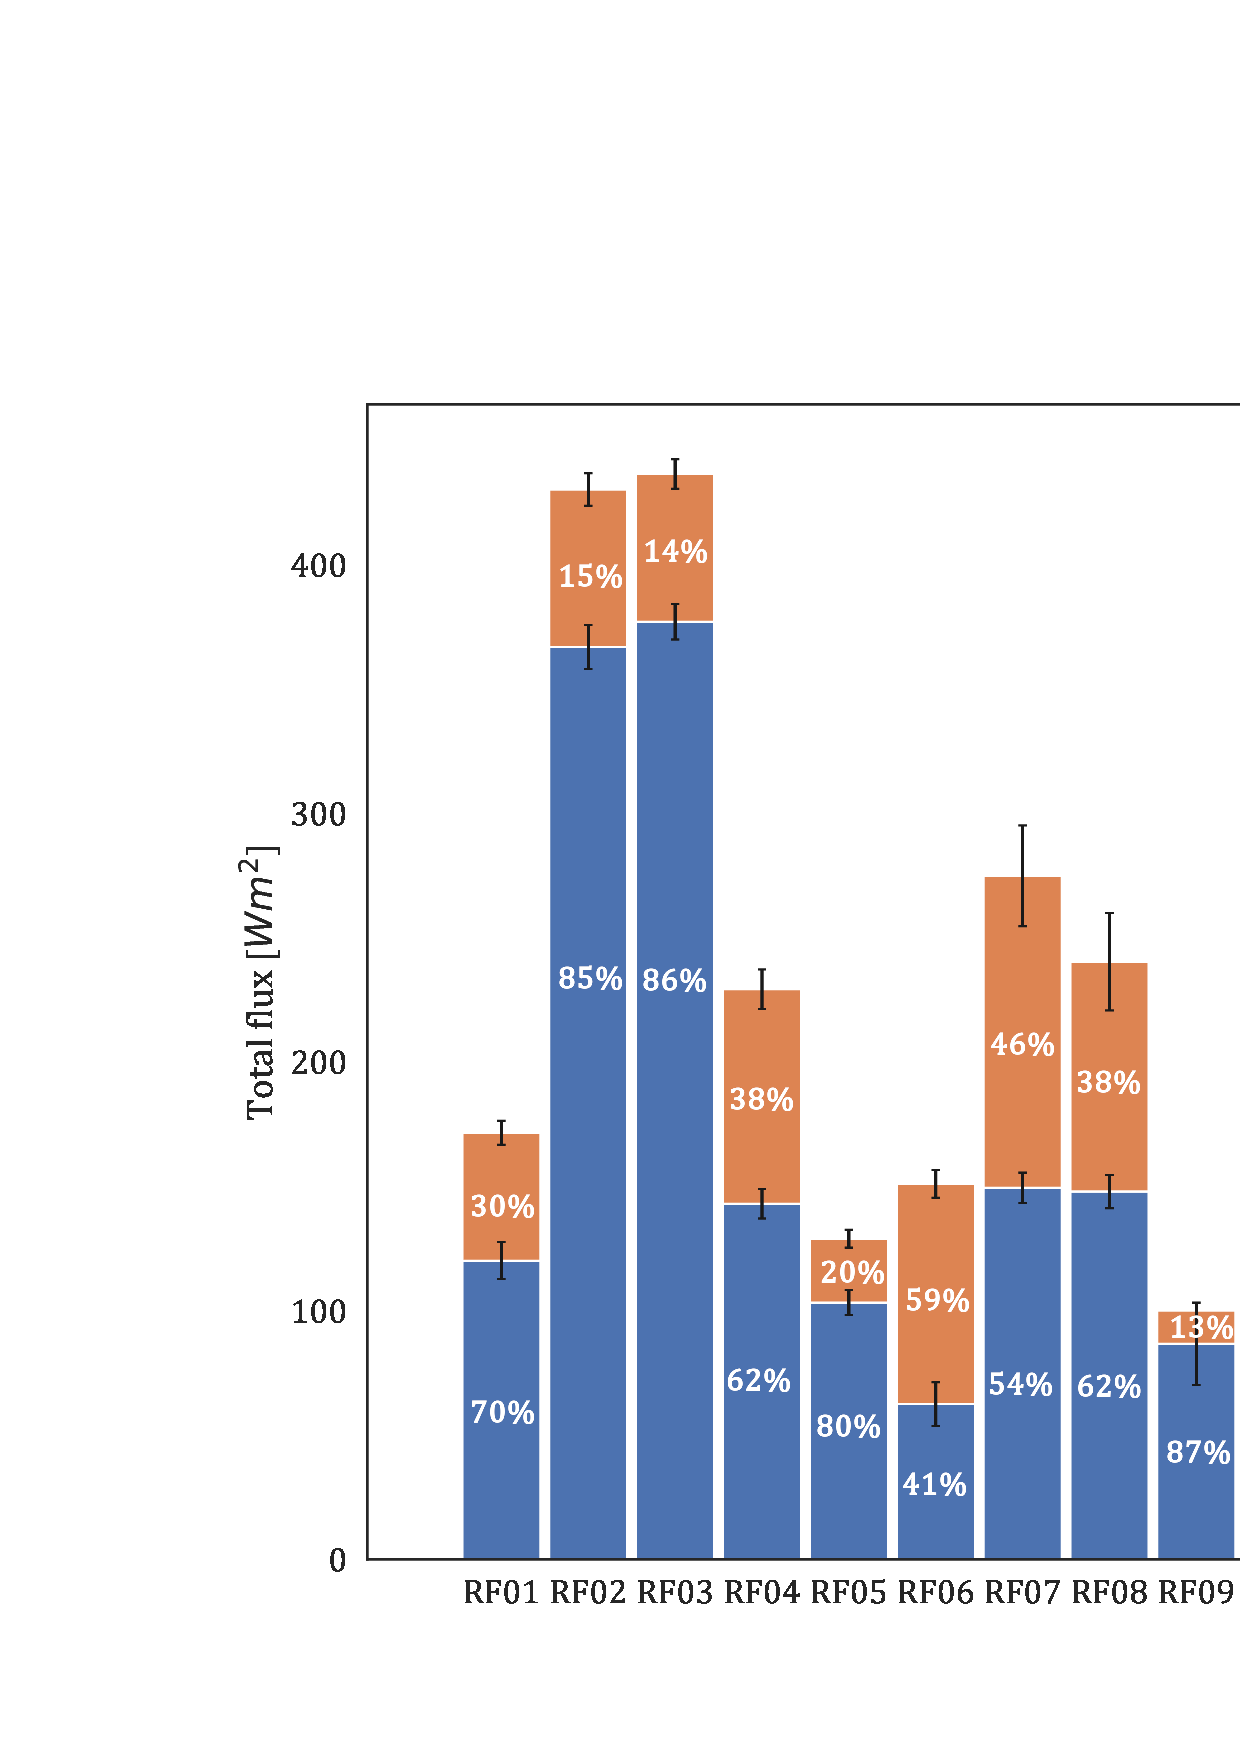
\includegraphics[width=\textwidth]{flight_100.png}
\caption{Total ( H + LE) fluxes measured on each research flight for all the processed research flight data. Each bar graph represents the mean, scale-resolved flux for a research flight. The x axis shows the research flights and y axis flux magnitudes. Turbulent fluxes in blue and mesoscale fluxes in orange. Percentage contributions in white numbers.}
\label{fig:flight_100}
\end{figure}

\newpage

\subsection{ABL and land surface drivers of transport}

\textbf{ABL dynamics}

\begin{figure}[hbtp]
 \noindent\includegraphics[width=\textwidth]{zL_IOP.png}
\caption{ Histograms of median $\zeta$ values for flight legs for all three IOPs}
\label{fig:zL_IOP}
\end{figure}
The turbulent surface layer scaling parameter $\zeta = \frac{z}{L}$, where z is the measurement height and L the Obukhov length, can be regarded as a stability parameter \cite{stull_introduction_1988}. Negative values of $\zeta$ close to 0 indicate a statically neutral surface layer and as the value decrease as the surface layer becomes more statically unstable. \\
Histograms of median $\zeta$ values from flight legs show that the August IOP is more convective than the other two IOPs with more data points within the  $\zeta$ $<$ -1 range (Figure \ref{fig:zL_IOP}). On the other hand the September IOP looks strongly shear driven, with most of the data falling within $\zeta$ $\in$ [-1 , 0). In this regard, July and September IOPs seem to be dynamically similar.


To understand how scale-resolved contributions vary with ABL dynamics, we looked at the PDFs of mesoscale fractions for shear driven ( $\zeta \in (-1,1]$  ) vs convectively driven ( $\zeta \in (-20,1]$  ) ABL (Figure \ref{fig:KDE_H_IOP}). The two distributions were found to have significantly different locations for all 3 IOPs using the Mann-Whitney U rank test with 95\% confidence. This indicates that there is a statistically significant higher fraction of mesoscale transport observed in convectively driven ABL across all the three IOPs.
\begin{figure}[hbtp]
 \noindent\includegraphics[width=\textwidth]{KDE_H_IOP.png}
\caption{ Kernal density estimates of sensible heat flux mesoscale fractions for all three IOPs}
\label{fig:KDE_H_IOP}
\end{figure}

For latent heat fluxes, the kernal density estimates of mesoscale fractions for the July and August IOPs show higher mesoscale fluxes for convective cases ( Figure \ref{fig:KDE_LE_IOP}). Performing a Mann-Whitney U rank test again showed that the distributions have significantly different values for the two stability regimes at 95\% confidence. However, for September IOP the mesoscale transport does not have a preference between a shear or convectively driven ABL. Even though July and September IOPs have similar ABL stability distributions their latent heat mesoscale transport does not show the same behaviour, hinting at the role of seasonality through changing surface characteristics and insolation. \begin{figure}[hbtp]
 \noindent\includegraphics[width=\textwidth]{KDE_LE_IOP.png}
\caption{ KDE plots of latent heat mesoscale fractions for all three IOPs}
\label{fig:KDE_LE_IOP}
\end{figure}

u*/w* is a non-dimensional parameter that can succinctly capture the competing effects of free and forced convection in the ABL. If the ABL is strongly shear driven, one would expect higher u* values and lower w* values, leading to higher values for u*/w* and vice versa for a convectively driven ABL. Kernel density estimates of u*/w* and the scatter of percentage mesoscale fluxes vs u*/w* reflect the $\zeta$ distribution characteristics for the 3 IOPs seen earlier in Figure \ref{fig:8}. September IOP has a median u*/w* value of 0.55, higher than the July ( 0.45 ) and August ( 0.43) IOPs, indicating more shear driven surface atmospheric transport. Similarly, the distributions for July and August IOPs are also similar with the august IOP having a slightly lower median value indicating more convectively driven transport.  
 \begin{figure}[hbtp]
 \noindent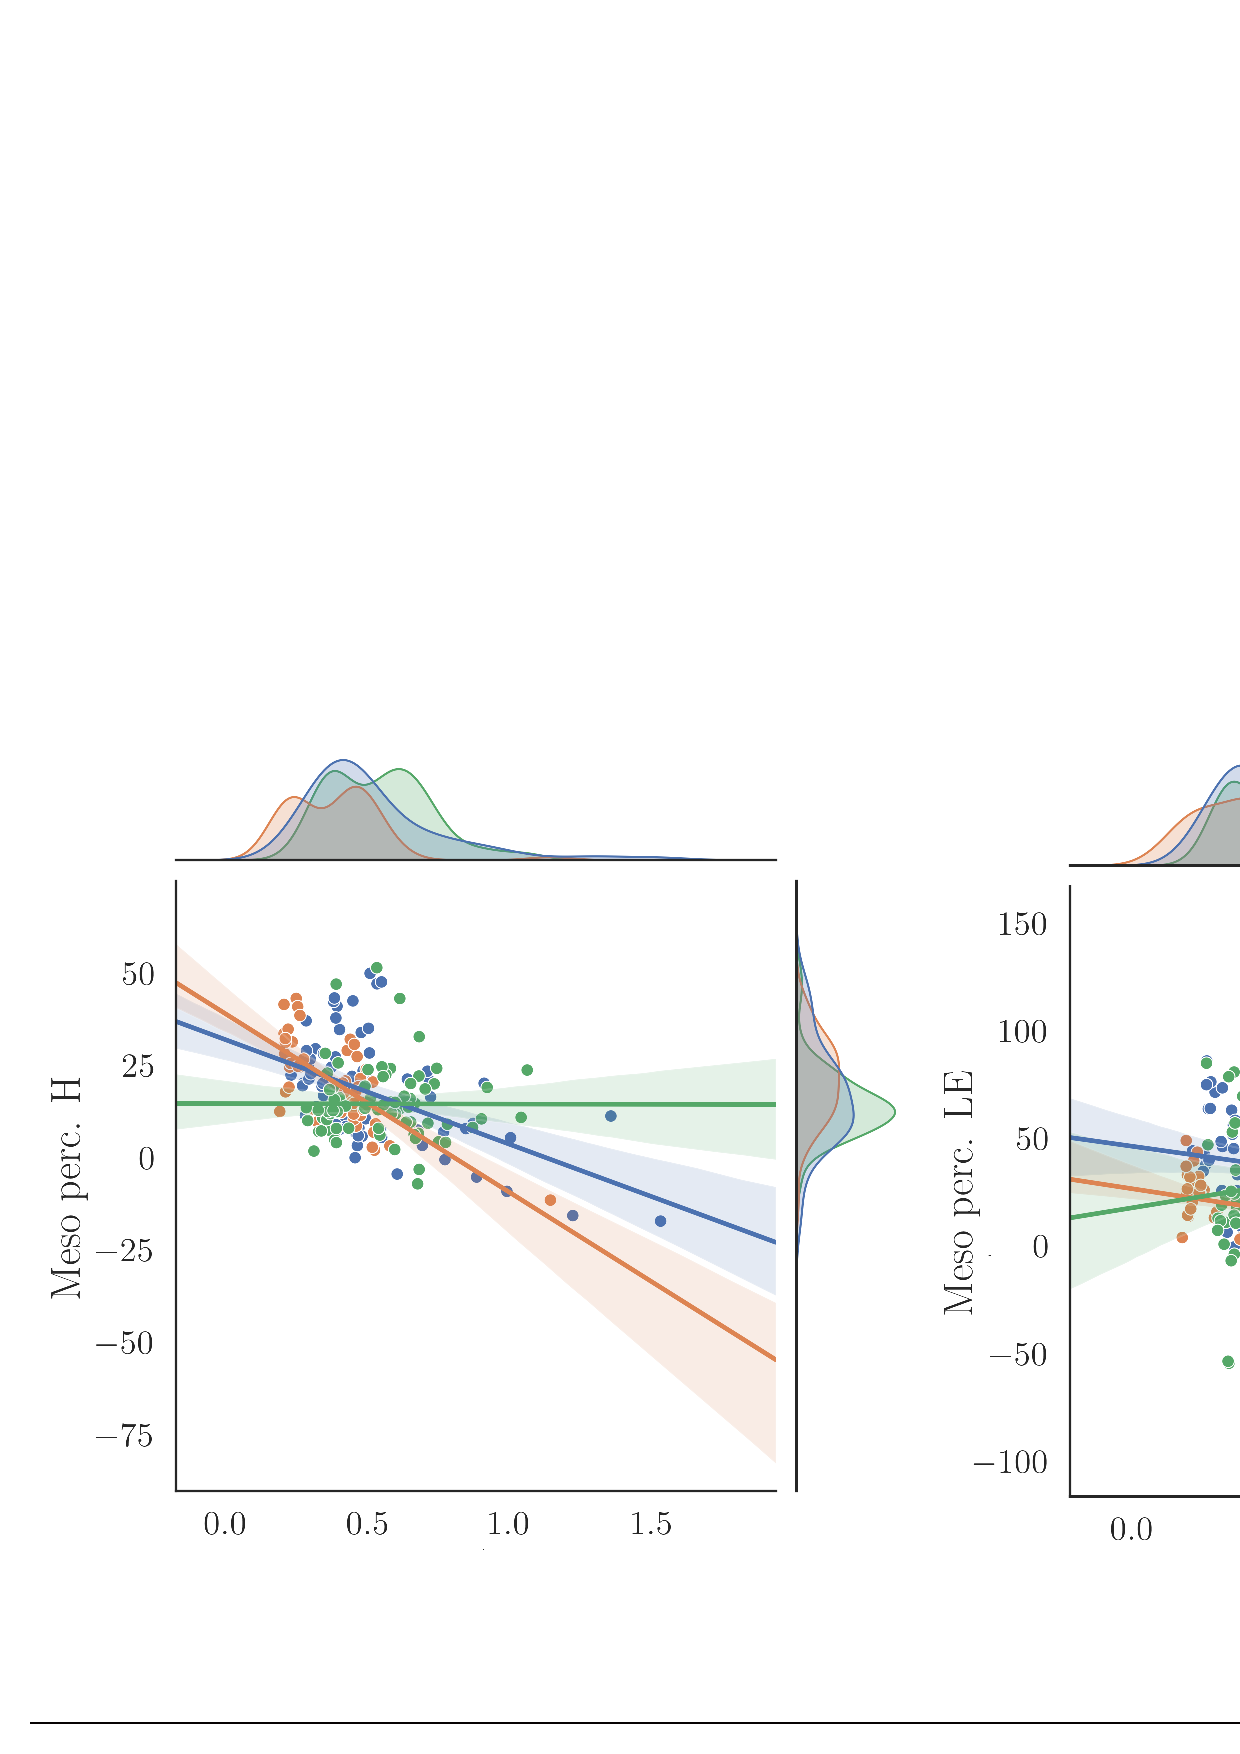
\includegraphics[width=\textwidth]{scatter_meso.png}
\caption{ Scatter plots of mesoscale flux percentages vs u*/w* for all three IOPs. Flight leg level averaged values are presented. Outlier removal was done for the mesoscale percentage values based on median absolute deviation (Boris Iglewicz and David Hoaglin 1993). Linear regression lines with 95\% confidence limits are also included for the same. Kernel Density Estimate plots for each distributions are drawn on their respective axes.}
\label{fig:scatter_meso}
 \end{figure}
 
The meso H percentages show a decreasing trend with increasing u*/w* values in July and August IOPs indicating higher mesoscale transport during more convective scenarios. This is especially clear in the almost flat regression line for the September IOP scatter. However, LE mes-scale flux percentages behave differently. For the September IOP they show and increasing trend with increasing values of u*/w*. Figure \ref{fig:4b} also shows high ( 29\%) mesoscale fluxes for LE in the September IOP. This once again illustrates that there is substantial mesoscale latent heat fluxes in both shear and convectively driven ABLs. The scatter of total ( H+ LE) mesoscale flux percentages gives a combined picture of the H and LE characteristics as seen from the first two plots in Figure \ref{fig:scatter_meso}. Here we see increasing mesoscale flux percentages for each IOP according to the dominant ABL stability, with increased contributions for convective cases in the July and August IOPs and for shear driven cases in the September IOP.  

\textbf{Distribution of land cover classes}

Most of the footprint contributions in the study domain comes from wetlands, coniferous and  broad leaf deciduous forests, with wetlands dominating the source areas (Figure \ref{fig:footprint_fraction} ). Further breaking down the wetland class, we find that most of the contributions come from the forested wetlands in the domain.

 \begin{figure}[hbtp]
 \noindent\includegraphics[width=\textwidth]{footprint_fraction.png}
\caption{ Fractional  footprint contributions for the major land cover classes within the study domain for each research flight.  Land cover class data from wiscland 2.0 database as shown in fig. 1 for the 40x40 km domain. Land cover classes have been grouped into open water, wetlands, deciduous forests, shrubs/grass/open land, coniferous and mixed forests.  The X axis shows the land cover class, and the Y axis rows are the airborne campaign dates. The numbers inside the boxes show fractional footprint contributions and they are also highlighted according to the color bar}
\label{fig:footprint_fraction}
 \end{figure}

\textbf{Flux contributions by land cover:}

 \begin{figure}[hbtp]
 \noindent\includegraphics[width=\textwidth]{footprint_IOP.png}
\caption{ Turbulent and mesoscale sensible and latent heat fluxes measured for the major land cover classes across the IOPs. For all research flights analysed, the land cover class with the maximum footprint contribution to the measured fluxes per flight leg was picked. Then this was grouped by their respective IOP. Turbulent fluxes in blue and mesoscale fluxes in orange. Panel a on top shows the LE fluxes and panel b at the bottom shows the H fluxes. Bar graphs for each of the three IOPs are separated by vertical dashed red lines and ordered as  contributions from coniferous, deciduous forests and wetlands within each IOP group }
\label{fig:footprint_IOP}
 \end{figure}
 
For a more detailed investigation of changes in footprint contributions with time, flight leg level footprint contributions were also calculated. This gave fractional footprint contributions for each flight leg from all the land cover classes. Using this data, the land cover class with the maximum fractional footprint contribution for each flight leg was picked. The same overall pattern across the IOPs seen in Figure 4 is repeated in Figure 12 as well, with regards to the magnitudes of the fluxes across IOPs and the scale-resolved percentages. The broadleaf deciduous forests have the lowest percentage turbulent fluxes in the July IOP, with only 37\% for LE and 70\% of H. \\
The kernel density estimates for mesoscale fractions did not show significant differences between the three major land cover classes.

\subsection{Space scale resolved fluxes}
 \begin{figure}[hbtp]
     \begin{subfigure}{0.85\textwidth}
         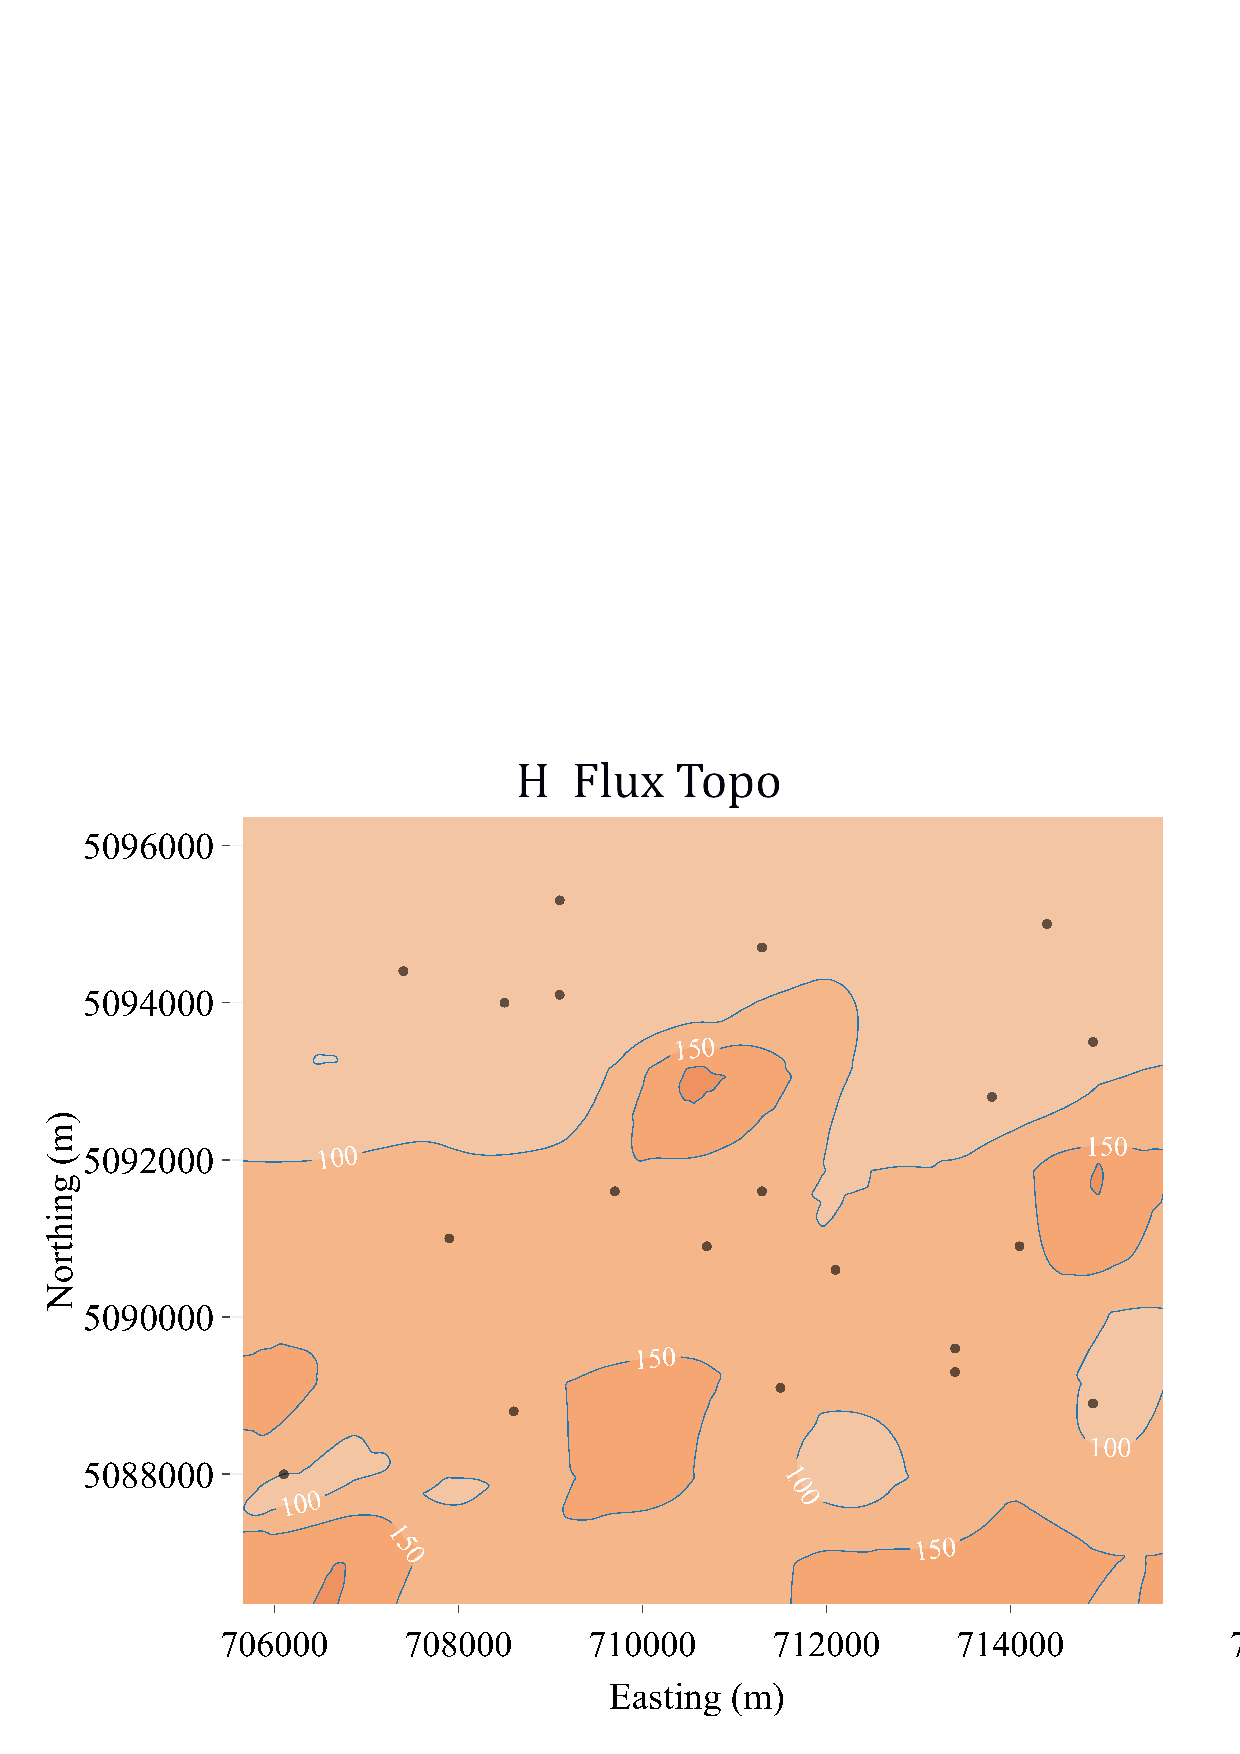
\includegraphics[width=1\textwidth]{topo_infi.png}
         \caption{Sensible and latent heat flux topographies }
         \label{fig:topo_infi}
     \end{subfigure}
     \begin{subfigure}{\textwidth}
         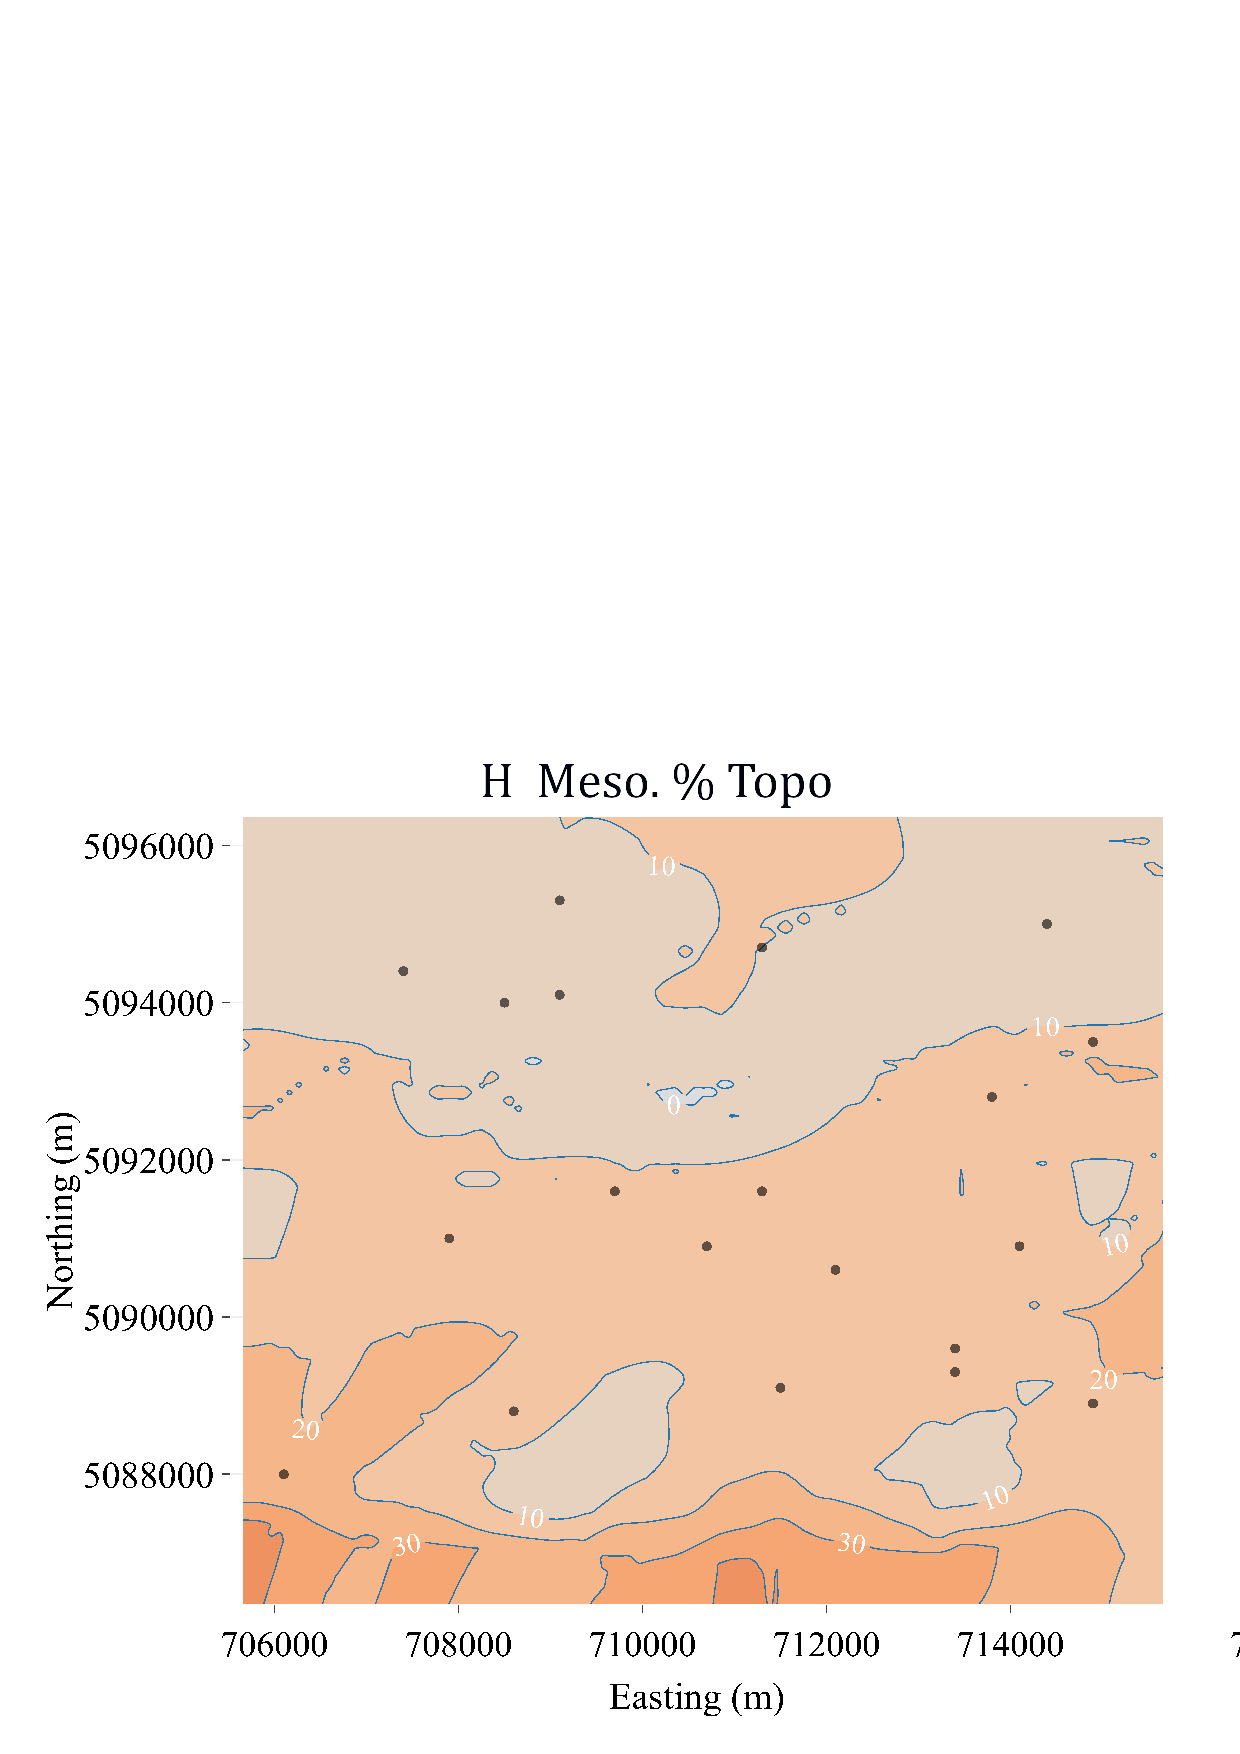
\includegraphics[width=0.85\textwidth]{topo_meso_perc.png}
         \caption{Percentage mesoscale contribution in the flux topographies}
         \label{fig:topo_meso_perc}
     \end{subfigure}
     \begin{subfigure}{\textwidth}
         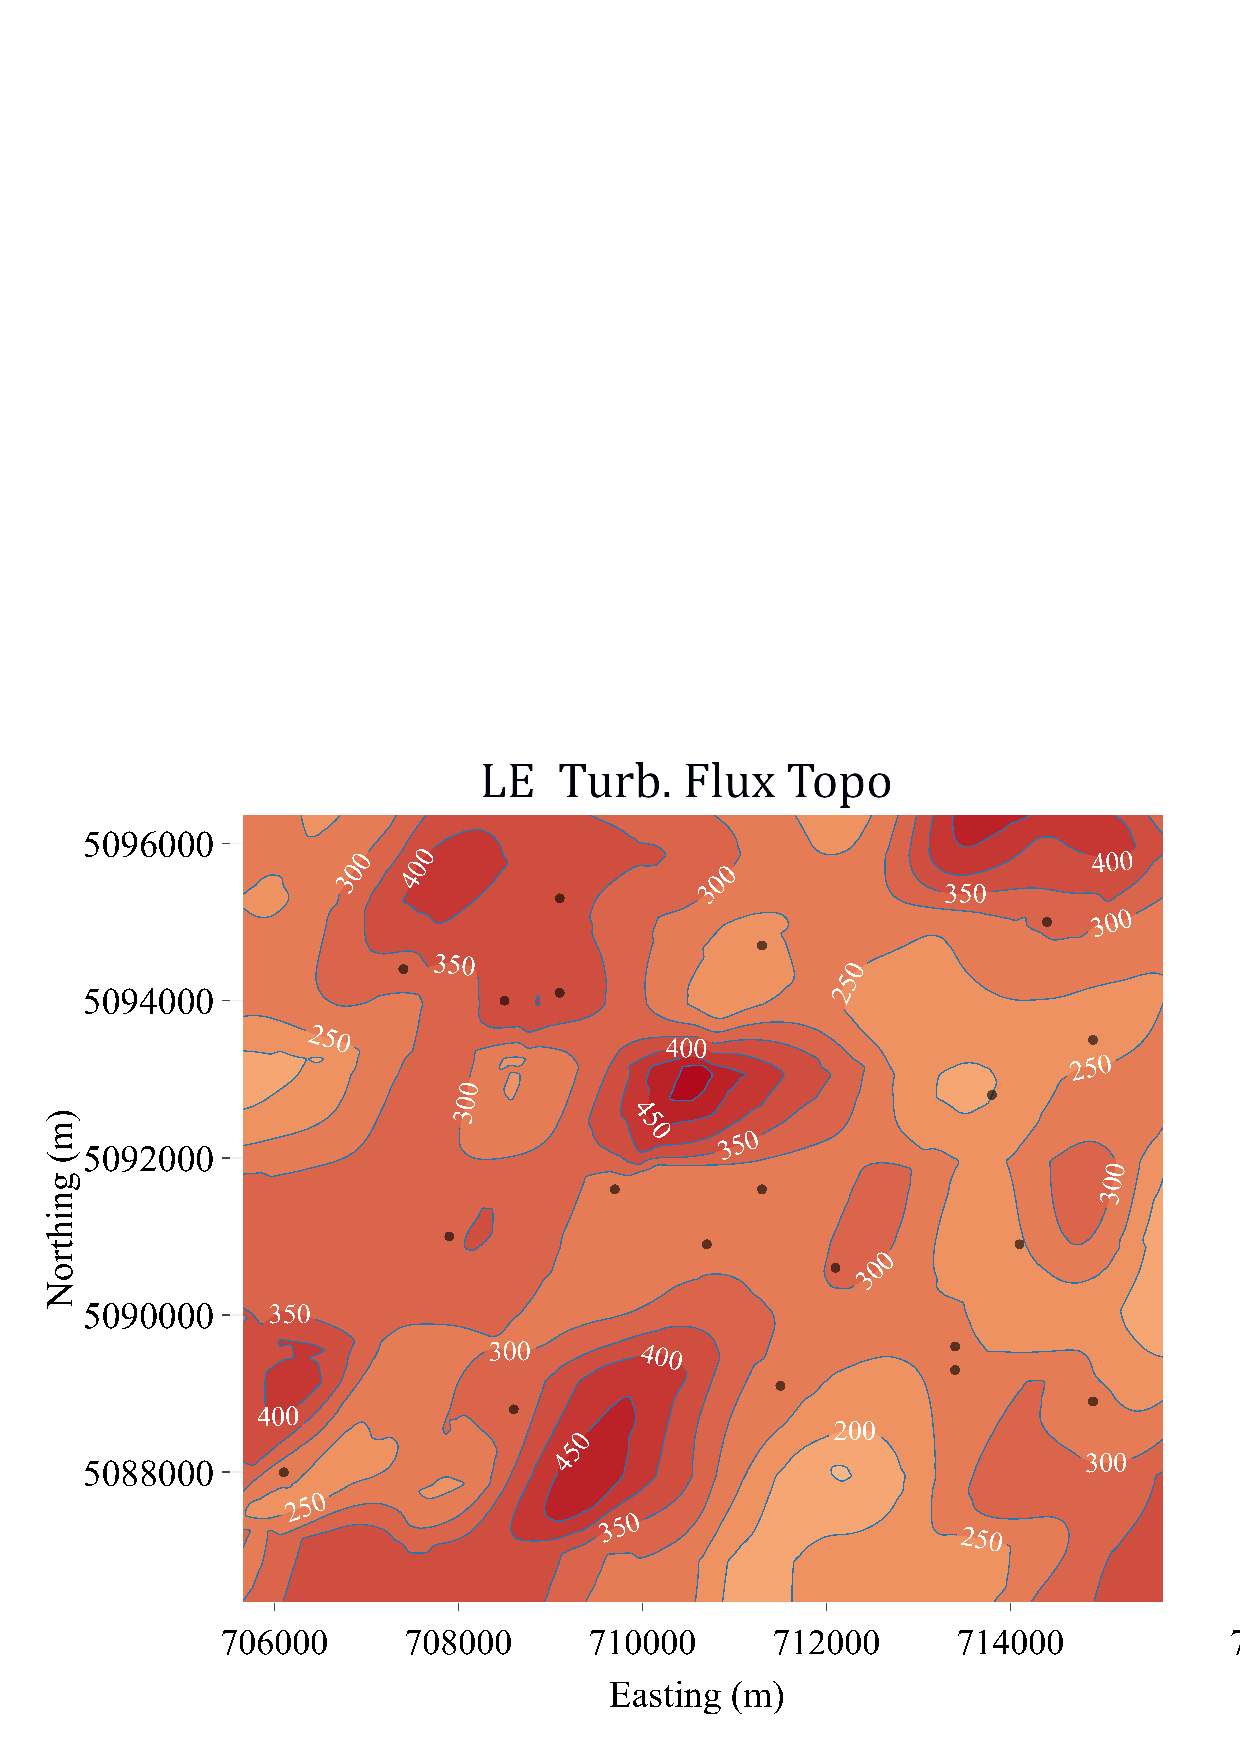
\includegraphics[width=0.85\textwidth]{topo_LE_turb_meso.png}
         \caption{Turbulent and mesoscale contributions of the latent heat flux topographies}
         \label{fig:topo_LE_turb_meso}
     \end{subfigure}
     \begin{subfigure}{\textwidth}
         \includegraphics[width=0.85\textwidth]{topo_LST_landcover.png}
         \caption{Surface properpties, LST (left, \cite{desai_multisensor_2021}) and land surface classes ( Wiscland 2.0) }
         \label{fig:topo_LST_land}
     \end{subfigure}
        \caption{Flux topographies for Research Flight 03 in the July IOP, 11 Jul. 09:20 to 11:20 CDT over the 10x10 km CHEESEHEAD core domain. The brown dots are the NCAR-ISFS. tower locations. (a) Sensible ( left) and latent ( right) heat flux topographies,(b) percentage mesoscale contributions to the sensible (left) and latent(right) heat flux topographies, (c) scale-resolved, turbulent (left) and mesoscale (right) topographies for the latent heat flux topo. in (a) and (d) distribution of land surface properties across the domain. }
        \label{fig:topo}
 \end{figure}
 
We present a case study for one good flight, with a sample flux topography for a summertime morning flight, RF03, conducted on July 11th, 2019 from 09:20 to 11:30 CDT. The flight did east -west transects across the domain, starting from the northern edge and moving to the south.  Aircraft logs for the day mention observing shallow cumulus clouds indicating local convection and weak winds for this day. This ensured that the flight transects had a good footprint coverage over the domain for this research flight. 

Spatially resolved sensible and latent heat flux topography maps ( Figure \ref{fig:topo_infi}) show similar order of magnitude values as  the IOP averaged behaviour in Figure \ref{fig:IOP_100}. The latent heat flux dominates and shows more spatial variability than the sensible heat flux. Spatial distribution patterns of both the fluxes not look similar either. The percentage mesoscale contributions for the two fluxes also show differing spatial patterns ( Figure \ref{fig:topo_meso_perc}). These flux topographies illustrate the fact that the CHEESEHEAD tower sites inside the study domain sample differing bowen ratios within the same 10x10 km domain and there are spatially varying , concomitant  mesoscale surface-atmospheric transport. This would imply that not all of the towers are sampling the same flux transport and the mesoscale transport associated with their locations would also be different. The flux topographies indicate stronger mesoscale contributions towards the southern edge of the domain in the sensible heat flux plots (Figure \ref{fig:topo_meso_perc}).This is due to the inherent time dependency in calculating the topographies from the flight transects. Each research flight duration is about 2 hours. This particular flight started measurements at the north end of the domain in early morning and by the time it reached the southern edge it was close to noon and by then a fully developed CBL would have formed. Sensible heat mesoscale fluxes develop more later in the day as well ( Figure \ref{fig:H_IOP01_diel}, \ref{fig:H_IOP02_diel}). The scale-resolved fluxes for latent heat for this flight indicate that the turbulent and meso peaks do not align in space ( Figure \ref{fig:topo_LE_turb_meso}). More flux topographies along with their standard error percentages ( Gantz et al.) are presented in the supplement. 

The inherent time dependency of the topographies leads to source strength non-stationarity, since the surface heat flux magnitudes change over the course of the measurement.This makes the flux topographies harder to interpret. A fusion LST product over the domain \cite{desai_multisensor_2021} for the measurement time shows a high amplitude west-east band in the centre (Figure \ref{fig:topo_LST_land}). mesoscale gradients can be observed close to this band in the latent heat flux plots of Figures 13.b and 13.c. However, since the large scale transport would be from quasi stationary structures we can't directly link the same to land cover or LST gradients in our current analysis framework. 

\newpage

\section{Discussion}

\textbf{Implications for Surface - Atmospheric Transport and Surface Energy Budget closure}

We observed higher fractions of  mesoscale transport for sensible and latent heat fluxes in convectively driven ABLs  as shown in the KDE plots (Figure \ref{fig:KDE_H_IOP} and Figure \ref{fig:KDE_LE_IOP}) in section 3.2. Previous observational studies have noted the inverse relationship between tower measured surface energy balance imbalance and u* \cite{stoy_data-driven_2013, eder_mesoscale_2015}, indicating that strong mechanical mixing in shear driven ABL leads to larger turbulent transport. Our findings also indicate the same, that lower frequency transport seems to have a preference for convectively driven boundary layers. The dependency of latent heat fluxes is more complicated than the sensible heat flux transport. 

Using data from the LITFASS 2003 field experiment in Germany \citeA{foken_energy_2008} \citeA{foken_energy_2010} showed that area averaged surface flux measurements reduce the surface energy budget residuals. This, combined with the observations that the residuals are worse for sites with more heterogeneous surfaces, leads to his hypothesis that what has remained unaccounted for in the budgets could be the transport due to quasi-stationary secondary circulations tied to landscape heterogeneity. The synthesis study by \citeA{stoy_data-driven_2013} found consistent energy balance non closures across the sites and more importantly, noted that non-closure is linked to the degree of landscape heterogeneity, quantified using MODIS products and GLOBEstat elevation data. Since then a growing body of research has suggested that quasi-stationary low-frequency eddies in the ABL tied to land surface heterogeneity can play an important role in surface-atmospheric transport.

LES studies with homogeneous \cite{salesky_nature_2017, li_coherent_2011} and heterogeneous (\citeA{margairaz_surface_2020}, idealised heterogeneities) surface forcings have observed secondary circulations in the ABL transition from convective rolls to a cellular structure as the ABL becomes more convectively unstable. \citeA{margairaz_surface_2020} notes that for their simulations, with imposed surface temperature heterogeneities in irregular rectangular patches, the convective-cell structure adjusts to the imposed surface temperature variations. The surface atmospheric transport associated with these circulations would be missed by tower based measurements unless they are either swept across the spatially-stationary measuring points by the mean wind or only if the point measurements happen to be in their vicinity \cite{mahrt_computing_2010, charuchittipan_extension_2014}.  These studies along with observations of better closure with longer averaging times and spatial measurements have led to a leading hypothesis that the surface energy balance closure problem is in fact a problem of scale \cite{foken_energy_2008, foken_energy_2010, mauder_surface-energy-balance_2020}

Large scale organisations in the form of longitudinal roll vortices, aligned with the mean wind can be generated in daytime convective boundary layers \cite{etling_roll_1993} while stationary circulations can also be induced by horizontal variations in surface roughness and heat flux \cite{desjardins_scaling_1997, sun_transport_1998} Blanford et al. (1991). LES studies have shown that over homogeneous surfaces, strongly unstable conditions can lead to the formation of standing convective cells akin to those that form in Rayleigh-Benard convection  \cite{kanda_les_2004, de_roo_influence_2018}. Over heterogeneous surfaces these free convective cells tend to become quasi-stationary secondary circulations, tied to the surface temperature, roughness or vegetation gradients \cite{inagaki_impact_2006, maronga_large-eddy_2013}. Such secondary circulation cells can lead to a persistent local-mean advective transport, leading to an underestimation of surface energy exchange \cite{morrison_impact_2021}

\cite{desai_multisensor_2021} presents a 50 m resolution fusion LST product for the same study domain, derived using a fusion of land surface model and satellite products. They note that the spatial standard deviation of the fusion product increases towards autumn and is also high for summer afternoons, with higher LST spatial gradients. This could be playing a role in the higher sensible heat mesoscale fluxes observed in the late morning and afternoon for the July and August IOPs (Figure \ref{fig:H_IOP01_diel} and \ref{fig:H_IOP02_diel} 5a,5c)

In this regard, using wavelet methods on high-frequency airborne data has allowed us to retain the larger scale surface-atmosphere transport across the heterogeneous study domain and account for relevant transport scales. The mesoscale contributions are not a fixed fraction of the total or turbulent fluxes but vary throughout the day and as the landscape undergoes seasonal transitions (Figure \ref{fig:IOP_100} and Figure \ref{fig:IOP_diel}). The scale-resolved sensible and latent heat fluxes do not behave similarly either. During the August IOP, (08/20 to 08/23), the measured bowen ratio is the lowest at 0.3 and this IOP has the lowest meso fraction for latent heat fluxes. Similarly, during the September IOP in early autumn ( 09/24 to 09/28) , the bowen ratio is the highest at 1.3 and mesoscale sensible heat flux fraction was the lowest during this IOP. The total mesoscale flux percentages for July IOP = 29\%, August IOP = 20\% and September IOP = 21\%. The total percentages are closer in magnitude because of the seasonal sensible and latent heat flux balance.  It is interesting to note that the August and September IOPs with very different bowen ratios have the same mesoscale flux percentages.

We also observed spatial variations of the mesoscale transport, which would not be sampled by stationary tower measurements within the domain (Figure \ref{fig:topo}, supplementary figure numbers). These flux topographies present a direct and physics-based flux map over the domain for the research flights analysed, providing a scale-resolved spatial distribution of sensible and latent heat fluxes. These topographies show persistent areas of large scale flux contributions within the study domain which could be linked to variations of land surface properties. However, the topographies are inherently limited by the foot prints of the airborne transects. The measured flux contributions can only be extrapolated within the flight transect footprints. Moreover the experimental design introduces a temporal element to the topographies. Even though spatially adjacent flight transects during a single flight are only about 6-8 minutes apart , a research flight across the domain takes about 2.5 hours. Since they don't represent a single snapshot in time, connecting the topographies with surface gradients can be complicated.

\section{Conclusions}

We present a systematic regional-scale observational analysis over a heterogeneous domain that quantifies the multi-scale nature of sub-grid scaling and patterning. The CHEESEHEAD19 field experiment provided a unique dataset to diagnose and quantify the diel and seasonal contributions from large scale transport over the study domain as its surface energy balance  shifts from a more latent heat flux-dominated late summer landscape to a more sensible heat flux-dominated early autumn landscape.

Using airborne measurements from this comprehensive field experiment dataset we sought to answer whether spatially resolved airborne eddy covariance can identify spatial scales of surface-atmosphere fluxes over heterogeneous surfaces?  Applying wavelet analysis to the airborne flux measurements from the field experiment data allowed us to spatially resolve and evaluate the mesoscale contributions at 100m above ground over the heterogeneous landscape. We looked at the diel and seasonal variability of the scale-resolved fluxes. The measured latent heat flux magnitudes had more pronounced seasonal changes than the sensible heat fluxes. We observed larger mesoscale transport for sensible heat fluxes in convectively driven ABL across the three IOP scenarios, while for latent heat fluxes only the July and August IOPs showed more fractional mesoscale transport in convectively driven ABLs. For the September IOP, which had mostly shear driven ABL cases, we did not find any significant change between the fractional mesoscale transport in convectively and shear driven ABLs. We hypothesise that the larger scale transport measured in our study could be linked to organized structures in the ABL as has been reported in previous numerical \cite{kanda_les_2004, inagaki_impact_2006, salesky_coherent_2020, margairaz_surface_2020} and observational \cite{eder_mesoscale_2015, morrison_impact_2021} studies. The flux topography case studies indicate that the mesoscale transport spatial variability would be missed by tower measurements in the domain. Areas of persistent contributions in the domain could be linked to the presence of co-located forested wetlands, creating roughness and thermal surface heterogeneities. 

From our observations and analyses we reject our null hypothesis that the mesoscale transport is an invariant, small fixed fraction of total flux. We conclude that our alternate hypothesis, persistent contributions of larger scale ( meso-$\beta$ to meso-$\gamma$ ) fluxes to the daytime sensible and latent heat fluxes exist with diurnal and seasonal variations, holds. However, with our current analysis we could not attribute the large scale fluxes to their sources or diagnose  quasi-stationary secondary circulations over the domain. This would require a space-time aligned dataset from high resolution numerical simulations like LES or products from scale aware scaling algorithms such as ERFs \cite{metzger_spatially_2013}.

The analysis helps further our understanding of the interactions between surface spatial heterogeneity and lower atmosphere feed-backs. Measurements of flux contributions over heterogeneous landscapes have not been studied well, in particular the shifts associated with seasonal landscape level transitions as is covered in this study. While the variation itself may not be an important component for synoptic and large scale weather dynamics, we believe that this adds a critical piece of information in assimilating and integrating observations and model outputs at multiple scales.

\section{Open Research}
AGU requires an Availability Statement for the underlying data needed to understand, evaluate, and build upon the reported research at the time of peer review and publication.

Authors should include an Availability Statement for the software that has a significant impact on the research. Details and templates are in the Availability Statement section of the Data and Software for Authors Guidance: \url{https://www.agu.org/Publish-with-AGU/Publish/Author-Resources/Data-and-Software-for-Authors#availability}

It is important to cite individual datasets in this section and, and they must be included in your bibliography. Please use the type field in your bibtex file to specify the type of data cited. Some options include Dataset, Software, Collection, ComputationalNotebook. Ex: 
\\
\begin{verbatim}

@misc{https://doi.org/10.7283/633e-1497,
  doi = {10.7283/633E-1497},
  url = {https://www.unavco.org/data/doi/10.7283/633E-1497},
  author = {de Zeeuw-van Dalfsen, Elske and Sleeman, Reinoud},
  title = {KNMI Dutch Antilles GPS Network - SAB1-St_Johns_Saba_NA P.S.},
  publisher = {UNAVCO, Inc.},
  year = {2019},
  type = {dataset}
}

\end{verbatim}

For physical samples, use the IGSN persistent identifier, see the International Geo Sample Numbers section:
\url{https://www.agu.org/Publish-with-AGU/Publish/Author-Resources/Data-and-Software-for-Authors#IGSN}
%%%%%%%%%%%%%%%%%%%%%%%%%%%%%%%%%%%%%%%%%%%%%%%

\acknowledgments
This material is based in part upon work supported by the National Science Foundation through the CHEESEHEAD19 project (grant no. AGS-1822420) and the NEON Program (grant no. DBI-0752017). The National Ecological Observatory Network is a program sponsored by the National Science Foundation and operated under cooperative agreement by Battelle. Brian Butterworth was additionally supported by the NOAA Physical Sciences Laboratory. We also recognize that our field research occurs on the traditional territories of the Ojibwe people, which have been unjustly ceded and whose ancestors were the original scientists and naturalists who stewarded the land, air, and waters we are fortunate to observe, reflect, and hopefully help continue to flourish.


%% ------------------------------------------------------------------------ %%
%% References and Citations

%%%%%%%%%%%%%%%%%%%%%%%%%%%%%%%%%%%%%%%%%%%%%%%
%
% \bibliography{<name of your .bib file>} don't specify the file extension
%
% don't specify bibliographystyle

% In the References section, cite the data/software described in the Availability Statement (this includes primary and processed data used for your research). For details on data/software citation as well as examples, see the Data & Software Citation section of the Data & Software for Authors guidance
% https://www.agu.org/Publish-with-AGU/Publish/Author-Resources/Data-and-Software-for-Authors#citation

%%%%%%%%%%%%%%%%%%%%%%%%%%%%%%%%%%%%%%%%%%%%%%%

\bibliography{paleri_library}



%Reference citation instructions and examples:
%
% Please use ONLY \cite and \citeA for reference citations.
% \cite for parenthetical references
% ...as shown in recent studies (Simpson et al., 2019)
% \citeA for in-text citations
% ...Simpson et al. (2019) have shown...
%
%
%...as shown by \citeA{jskilby}.
%...as shown by \citeA{lewin76}, \citeA{carson86}, \citeA{bartoldy02}, and \citeA{rinaldi03}.
%...has been shown \cite{jskilbye}.
%...has been shown \cite{lewin76,carson86,bartoldy02,rinaldi03}.
%... \cite <i.e.>[]{lewin76,carson86,bartoldy02,rinaldi03}.
%...has been shown by \cite <e.g.,>[and others]{lewin76}.
%
% apacite uses < > for prenotes and [ ] for postnotes
% DO NOT use other cite commands (e.g., \citet, \citep, \citeyear, \citealp, etc.).
% \nocite is okay to use to add references from your Supporting Information
%



\end{document}



More Information and Advice:

%% ------------------------------------------------------------------------ %%
%
%  SECTION HEADS
%
%% ------------------------------------------------------------------------ %%

% Capitalize the first letter of each word (except for
% prepositions, conjunctions, and articles that are
% three or fewer letters).

% AGU follows standard outline style; therefore, there cannot be a section 1 without
% a section 2, or a section 2.3.1 without a section 2.3.2.
% Please make sure your section numbers are balanced.
% ---------------
% Level 1 head
%
% Use the \section{} command to identify level 1 heads;
% type the appropriate head wording between the curly
% brackets, as shown below.
%
%An example:
%\section{Level 1 Head: Introduction}
%
% ---------------
% Level 2 head
%
% Use the \subsection{} command to identify level 2 heads.
%An example:
%\subsection{Level 2 Head}
%
% ---------------
% Level 3 head
%
% Use the \subsubsection{} command to identify level 3 heads
%An example:
%\subsubsection{Level 3 Head}
%
%---------------
% Level 4 head
%
% Use the \subsubsubsection{} command to identify level 3 heads
% An example:
%\subsubsubsection{Level 4 Head} An example.
%
%% ------------------------------------------------------------------------ %%
%
%  IN-TEXT LISTS
%
%% ------------------------------------------------------------------------ %%
%
% Do not use bulleted lists; enumerated lists are okay.
% \begin{enumerate}
% \item
% \item
% \item
% \end{enumerate}
%
%% ------------------------------------------------------------------------ %%
%
%  EQUATIONS
%
%% ------------------------------------------------------------------------ %%

% Single-line equations are centered.
% Equation arrays will appear left-aligned.

Math coded inside display math mode \[ ...\]
 will not be numbered, e.g.,:
 \[ x^2=y^2 + z^2\]

 Math coded inside \begin{equation} and \end{equation} will
 be automatically numbered, e.g.,:
 \begin{equation}
 x^2=y^2 + z^2
 \end{equation}


% To create multiline equations, use the
% \begin{eqnarray} and \end{eqnarray} environment
% as demonstrated below.
\begin{eqnarray}
  x_{1} & = & (x - x_{0}) \cos \Theta \nonumber \\
        && + (y - y_{0}) \sin \Theta  \nonumber \\
  y_{1} & = & -(x - x_{0}) \sin \Theta \nonumber \\
        && + (y - y_{0}) \cos \Theta.
\end{eqnarray}

%If you don't want an equation number, use the star form:
%\begin{eqnarray*}...\end{eqnarray*}

% Break each line at a sign of operation
% (+, -, etc.) if possible, with the sign of operation
% on the new line.

% Indent second and subsequent lines to align with
% the first character following the equal sign on the
% first line.

% Use an \hspace{} command to insert horizontal space
% into your equation if necessary. Place an appropriate
% unit of measure between the curly braces, e.g.
% \hspace{1in}; you may have to experiment to achieve
% the correct amount of space.


%% ------------------------------------------------------------------------ %%
%
%  EQUATION NUMBERING: COUNTER
%
%% ------------------------------------------------------------------------ %%

% You may change equation numbering by resetting
% the equation counter or by explicitly numbering
% an equation.

% To explicitly number an equation, type \eqnum{}
% (with the desired number between the brackets)
% after the \begin{equation} or \begin{eqnarray}
% command.  The \eqnum{} command will affect only
% the equation it appears with; LaTeX will number
% any equations appearing later in the manuscript
% according to the equation counter.
%

% If you have a multiline equation that needs only
% one equation number, use a \nonumber command in
% front of the double backslashes (\\) as shown in
% the multiline equation above.

% If you are using line numbers, remember to surround
% equations with \begin{linenomath*}...\end{linenomath*}

%  To add line numbers to lines in equations:
%  \begin{linenomath*}
%  \begin{equation}
%  \end{equation}
%  \end{linenomath*}



